\documentclass[twoside]{book}

% Packages required by doxygen
\usepackage{calc}
\usepackage{doxygen}
\usepackage{graphicx}
\usepackage[utf8]{inputenc}
\usepackage{makeidx}
\usepackage{multicol}
\usepackage{multirow}
\usepackage{textcomp}
\usepackage[table]{xcolor}

% Font selection
\usepackage[T1]{fontenc}
\usepackage{mathptmx}
\usepackage[scaled=.90]{helvet}
\usepackage{courier}
\usepackage{amssymb}
\usepackage{sectsty}
\renewcommand{\familydefault}{\sfdefault}
\allsectionsfont{%
  \fontseries{bc}\selectfont%
  \color{darkgray}%
}
\renewcommand{\DoxyLabelFont}{%
  \fontseries{bc}\selectfont%
  \color{darkgray}%
}

% Page & text layout
\usepackage{geometry}
\geometry{%
  a4paper,%
  top=2.5cm,%
  bottom=2.5cm,%
  left=2.5cm,%
  right=2.5cm%
}
\tolerance=750
\hfuzz=15pt
\hbadness=750
\setlength{\emergencystretch}{15pt}
\setlength{\parindent}{0cm}
\setlength{\parskip}{0.2cm}
\makeatletter
\renewcommand{\paragraph}{%
  \@startsection{paragraph}{4}{0ex}{-1.0ex}{1.0ex}{%
    \normalfont\normalsize\bfseries\SS@parafont%
  }%
}
\renewcommand{\subparagraph}{%
  \@startsection{subparagraph}{5}{0ex}{-1.0ex}{1.0ex}{%
    \normalfont\normalsize\bfseries\SS@subparafont%
  }%
}
\makeatother

% Headers & footers
\usepackage{fancyhdr}
\pagestyle{fancyplain}
\fancyhead[LE]{\fancyplain{}{\bfseries\thepage}}
\fancyhead[CE]{\fancyplain{}{}}
\fancyhead[RE]{\fancyplain{}{\bfseries\leftmark}}
\fancyhead[LO]{\fancyplain{}{\bfseries\rightmark}}
\fancyhead[CO]{\fancyplain{}{}}
\fancyhead[RO]{\fancyplain{}{\bfseries\thepage}}
\fancyfoot[LE]{\fancyplain{}{}}
\fancyfoot[CE]{\fancyplain{}{}}
\fancyfoot[RE]{\fancyplain{}{\bfseries\scriptsize Generated on Thu Apr 10 2014 09\-:43\-:49 for Mind\-Chair by Doxygen }}
\fancyfoot[LO]{\fancyplain{}{\bfseries\scriptsize Generated on Thu Apr 10 2014 09\-:43\-:49 for Mind\-Chair by Doxygen }}
\fancyfoot[CO]{\fancyplain{}{}}
\fancyfoot[RO]{\fancyplain{}{}}
\renewcommand{\footrulewidth}{0.4pt}
\renewcommand{\chaptermark}[1]{%
  \markboth{#1}{}%
}
\renewcommand{\sectionmark}[1]{%
  \markright{\thesection\ #1}%
}

% Indices & bibliography
\usepackage{natbib}
\usepackage[titles]{tocloft}
\setcounter{tocdepth}{3}
\setcounter{secnumdepth}{5}
\makeindex

% Hyperlinks (required, but should be loaded last)
\usepackage{ifpdf}
\ifpdf
  \usepackage[pdftex,pagebackref=true]{hyperref}
\else
  \usepackage[ps2pdf,pagebackref=true]{hyperref}
\fi
\hypersetup{%
  colorlinks=true,%
  linkcolor=blue,%
  citecolor=blue,%
  unicode%
}

% Custom commands
\newcommand{\clearemptydoublepage}{%
  \newpage{\pagestyle{empty}\cleardoublepage}%
}


%===== C O N T E N T S =====

\begin{document}

% Titlepage & ToC
\hypersetup{pageanchor=false}
\pagenumbering{roman}
\begin{titlepage}
\vspace*{7cm}
\begin{center}%
{\Large Mind\-Chair }\\
\vspace*{1cm}
{\large Generated by Doxygen 1.8.5}\\
\vspace*{0.5cm}
{\small Thu Apr 10 2014 09:43:49}\\
\end{center}
\end{titlepage}
\clearemptydoublepage
\tableofcontents
\clearemptydoublepage
\pagenumbering{arabic}
\hypersetup{pageanchor=true}

%--- Begin generated contents ---
\chapter{Deprecated List}
\label{deprecated}
\hypertarget{deprecated}{}

\begin{DoxyRefList}
\item[\label{deprecated__deprecated000002}%
\hypertarget{deprecated__deprecated000002}{}%
Member \hyperlink{classgui_1_1_g_u_i_a8912704162cb5ae17664a4f5f13297a6}{gui.G\-U\-I.lightensor\-Error} (Position position)]use \hyperlink{}{show\-Error\-Pop\-Up(\-String message)} instead  
\item[\label{deprecated__deprecated000001}%
\hypertarget{deprecated__deprecated000001}{}%
Member \hyperlink{classgui_1_1_g_u_i_a680939303c766a1d1b1c86dcfd074255}{gui.G\-U\-I.light\-Sensor\-Alright} (Position position)]use \hyperlink{}{show\-Alright\-Pop\-Up(\-String message)} instead 
\end{DoxyRefList}
\chapter{Namespace Index}
\section{Packages}
Here are the packages with brief descriptions (if available)\-:\begin{DoxyCompactList}
\item\contentsline{section}{\hyperlink{namespacecontrollers}{controllers} }{\pageref{namespacecontrollers}}{}
\item\contentsline{section}{\hyperlink{namespacegui}{gui} }{\pageref{namespacegui}}{}
\item\contentsline{section}{\hyperlink{namespacemotors}{motors} }{\pageref{namespacemotors}}{}
\item\contentsline{section}{\hyperlink{namespacenxt}{nxt} }{\pageref{namespacenxt}}{}
\item\contentsline{section}{\hyperlink{namespacesensors}{sensors} }{\pageref{namespacesensors}}{}
\end{DoxyCompactList}

\chapter{Hierarchical Index}
\section{Class Hierarchy}
This inheritance list is sorted roughly, but not completely, alphabetically\-:\begin{DoxyCompactList}
\item \contentsline{section}{controllers.\-Calibration\-Controller}{\pageref{classcontrollers_1_1_calibration_controller}}{}
\item Color\-Sensor\begin{DoxyCompactList}
\item \contentsline{section}{sensors.\-My\-Color\-Sensor}{\pageref{classsensors_1_1_my_color_sensor}}{}
\end{DoxyCompactList}
\item \contentsline{section}{gui.\-G\-U\-I}{\pageref{classgui_1_1_g_u_i}}{}
\item \contentsline{section}{gui.\-Icons}{\pageref{enumgui_1_1_icons}}{}
\item Light\-Sensor\begin{DoxyCompactList}
\item \contentsline{section}{sensors.\-My\-Light\-Sensor}{\pageref{classsensors_1_1_my_light_sensor}}{}
\end{DoxyCompactList}
\item \contentsline{section}{sensors.\-Light\-Sensor\-Listener}{\pageref{interfacesensors_1_1_light_sensor_listener}}{}
\begin{DoxyCompactList}
\item \contentsline{section}{controllers.\-Line\-Follow\-Controller}{\pageref{classcontrollers_1_1_line_follow_controller}}{}
\item \contentsline{section}{controllers.\-Obstruction\-Controller}{\pageref{classcontrollers_1_1_obstruction_controller}}{}
\end{DoxyCompactList}
\item \contentsline{section}{nxt.\-Main}{\pageref{classnxt_1_1_main}}{}
\item \contentsline{section}{motors.\-Motor\-Controller}{\pageref{classmotors_1_1_motor_controller}}{}
\item \contentsline{section}{sensors.\-Position}{\pageref{enumsensors_1_1_position}}{}
\item Runnable\begin{DoxyCompactList}
\item \contentsline{section}{controllers.\-Obstruction\-Controller}{\pageref{classcontrollers_1_1_obstruction_controller}}{}
\end{DoxyCompactList}
\item \contentsline{section}{sensors.\-Sensor\-Type}{\pageref{enumsensors_1_1_sensor_type}}{}
\item Thread\begin{DoxyCompactList}
\item \contentsline{section}{controllers.\-Line\-Follow\-Controller}{\pageref{classcontrollers_1_1_line_follow_controller}}{}
\item \contentsline{section}{sensors.\-Sensor\-Handler}{\pageref{classsensors_1_1_sensor_handler}}{}
\end{DoxyCompactList}
\item Ultrasonic\-Sensor\begin{DoxyCompactList}
\item \contentsline{section}{sensors.\-My\-Ultra\-Sonic\-Sensor}{\pageref{classsensors_1_1_my_ultra_sonic_sensor}}{}
\end{DoxyCompactList}
\item \contentsline{section}{sensors.\-Ultrasonic\-Sensor\-Listener}{\pageref{interfacesensors_1_1_ultrasonic_sensor_listener}}{}
\begin{DoxyCompactList}
\item \contentsline{section}{controllers.\-Obstruction\-Controller}{\pageref{classcontrollers_1_1_obstruction_controller}}{}
\end{DoxyCompactList}
\item \contentsline{section}{sensors.\-Updating\-Sensor}{\pageref{interfacesensors_1_1_updating_sensor}}{}
\begin{DoxyCompactList}
\item \contentsline{section}{sensors.\-My\-Color\-Sensor}{\pageref{classsensors_1_1_my_color_sensor}}{}
\item \contentsline{section}{sensors.\-My\-Light\-Sensor}{\pageref{classsensors_1_1_my_light_sensor}}{}
\item \contentsline{section}{sensors.\-My\-Ultra\-Sonic\-Sensor}{\pageref{classsensors_1_1_my_ultra_sonic_sensor}}{}
\end{DoxyCompactList}
\end{DoxyCompactList}

\chapter{Class Index}
\section{Class List}
Here are the classes, structs, unions and interfaces with brief descriptions\-:\begin{DoxyCompactList}
\item\contentsline{section}{\hyperlink{classcontrollers_1_1_calibration_controller}{controllers.\-Calibration\-Controller} }{\pageref{classcontrollers_1_1_calibration_controller}}{}
\item\contentsline{section}{\hyperlink{classgui_1_1_g_u_i}{gui.\-G\-U\-I} }{\pageref{classgui_1_1_g_u_i}}{}
\item\contentsline{section}{\hyperlink{enumgui_1_1_icons}{gui.\-Icons} }{\pageref{enumgui_1_1_icons}}{}
\item\contentsline{section}{\hyperlink{interfacesensors_1_1_light_sensor_listener}{sensors.\-Light\-Sensor\-Listener} }{\pageref{interfacesensors_1_1_light_sensor_listener}}{}
\item\contentsline{section}{\hyperlink{classcontrollers_1_1_line_follow_controller}{controllers.\-Line\-Follow\-Controller} }{\pageref{classcontrollers_1_1_line_follow_controller}}{}
\item\contentsline{section}{\hyperlink{classnxt_1_1_main}{nxt.\-Main} }{\pageref{classnxt_1_1_main}}{}
\item\contentsline{section}{\hyperlink{classmotors_1_1_motor_controller}{motors.\-Motor\-Controller} }{\pageref{classmotors_1_1_motor_controller}}{}
\item\contentsline{section}{\hyperlink{classsensors_1_1_my_color_sensor}{sensors.\-My\-Color\-Sensor} }{\pageref{classsensors_1_1_my_color_sensor}}{}
\item\contentsline{section}{\hyperlink{classsensors_1_1_my_light_sensor}{sensors.\-My\-Light\-Sensor} }{\pageref{classsensors_1_1_my_light_sensor}}{}
\item\contentsline{section}{\hyperlink{classsensors_1_1_my_ultra_sonic_sensor}{sensors.\-My\-Ultra\-Sonic\-Sensor} }{\pageref{classsensors_1_1_my_ultra_sonic_sensor}}{}
\item\contentsline{section}{\hyperlink{classcontrollers_1_1_obstruction_controller}{controllers.\-Obstruction\-Controller} }{\pageref{classcontrollers_1_1_obstruction_controller}}{}
\item\contentsline{section}{\hyperlink{enumsensors_1_1_position}{sensors.\-Position} }{\pageref{enumsensors_1_1_position}}{}
\item\contentsline{section}{\hyperlink{classsensors_1_1_sensor_handler}{sensors.\-Sensor\-Handler} }{\pageref{classsensors_1_1_sensor_handler}}{}
\item\contentsline{section}{\hyperlink{enumsensors_1_1_sensor_type}{sensors.\-Sensor\-Type} }{\pageref{enumsensors_1_1_sensor_type}}{}
\item\contentsline{section}{\hyperlink{interfacesensors_1_1_ultrasonic_sensor_listener}{sensors.\-Ultrasonic\-Sensor\-Listener} }{\pageref{interfacesensors_1_1_ultrasonic_sensor_listener}}{}
\item\contentsline{section}{\hyperlink{interfacesensors_1_1_updating_sensor}{sensors.\-Updating\-Sensor} }{\pageref{interfacesensors_1_1_updating_sensor}}{}
\end{DoxyCompactList}

\chapter{File Index}
\section{File List}
Here is a list of all files with brief descriptions\-:\begin{DoxyCompactList}
\item\contentsline{section}{C\-:/\-Users/hp/git/the\-End/\-Eind\-Project/src/controllers/\hyperlink{_calibration_controller_8java}{Calibration\-Controller.\-java} }{\pageref{_calibration_controller_8java}}{}
\item\contentsline{section}{C\-:/\-Users/hp/git/the\-End/\-Eind\-Project/src/controllers/\hyperlink{_line_follow_controller_8java}{Line\-Follow\-Controller.\-java} }{\pageref{_line_follow_controller_8java}}{}
\item\contentsline{section}{C\-:/\-Users/hp/git/the\-End/\-Eind\-Project/src/controllers/\hyperlink{_obstruction_controller_8java}{Obstruction\-Controller.\-java} }{\pageref{_obstruction_controller_8java}}{}
\item\contentsline{section}{C\-:/\-Users/hp/git/the\-End/\-Eind\-Project/src/gui/\hyperlink{_g_u_i_8java}{G\-U\-I.\-java} }{\pageref{_g_u_i_8java}}{}
\item\contentsline{section}{C\-:/\-Users/hp/git/the\-End/\-Eind\-Project/src/gui/\hyperlink{_icons_8java}{Icons.\-java} }{\pageref{_icons_8java}}{}
\item\contentsline{section}{C\-:/\-Users/hp/git/the\-End/\-Eind\-Project/src/motors/\hyperlink{_motor_controller_8java}{Motor\-Controller.\-java} }{\pageref{_motor_controller_8java}}{}
\item\contentsline{section}{C\-:/\-Users/hp/git/the\-End/\-Eind\-Project/src/nxt/\hyperlink{_main_8java}{Main.\-java} }{\pageref{_main_8java}}{}
\item\contentsline{section}{C\-:/\-Users/hp/git/the\-End/\-Eind\-Project/src/sensors/\hyperlink{_light_sensor_listener_8java}{Light\-Sensor\-Listener.\-java} }{\pageref{_light_sensor_listener_8java}}{}
\item\contentsline{section}{C\-:/\-Users/hp/git/the\-End/\-Eind\-Project/src/sensors/\hyperlink{_my_color_sensor_8java}{My\-Color\-Sensor.\-java} }{\pageref{_my_color_sensor_8java}}{}
\item\contentsline{section}{C\-:/\-Users/hp/git/the\-End/\-Eind\-Project/src/sensors/\hyperlink{_my_light_sensor_8java}{My\-Light\-Sensor.\-java} }{\pageref{_my_light_sensor_8java}}{}
\item\contentsline{section}{C\-:/\-Users/hp/git/the\-End/\-Eind\-Project/src/sensors/\hyperlink{_my_ultra_sonic_sensor_8java}{My\-Ultra\-Sonic\-Sensor.\-java} }{\pageref{_my_ultra_sonic_sensor_8java}}{}
\item\contentsline{section}{C\-:/\-Users/hp/git/the\-End/\-Eind\-Project/src/sensors/\hyperlink{_position_8java}{Position.\-java} }{\pageref{_position_8java}}{}
\item\contentsline{section}{C\-:/\-Users/hp/git/the\-End/\-Eind\-Project/src/sensors/\hyperlink{_sensor_handler_8java}{Sensor\-Handler.\-java} }{\pageref{_sensor_handler_8java}}{}
\item\contentsline{section}{C\-:/\-Users/hp/git/the\-End/\-Eind\-Project/src/sensors/\hyperlink{_sensor_type_8java}{Sensor\-Type.\-java} }{\pageref{_sensor_type_8java}}{}
\item\contentsline{section}{C\-:/\-Users/hp/git/the\-End/\-Eind\-Project/src/sensors/\hyperlink{_ultrasonic_sensor_listener_8java}{Ultrasonic\-Sensor\-Listener.\-java} }{\pageref{_ultrasonic_sensor_listener_8java}}{}
\item\contentsline{section}{C\-:/\-Users/hp/git/the\-End/\-Eind\-Project/src/sensors/\hyperlink{_updating_sensor_8java}{Updating\-Sensor.\-java} }{\pageref{_updating_sensor_8java}}{}
\end{DoxyCompactList}

\chapter{Namespace Documentation}
\hypertarget{namespacecontrollers}{\section{Package controllers}
\label{namespacecontrollers}\index{controllers@{controllers}}
}
\subsection*{Classes}
\begin{DoxyCompactItemize}
\item 
class \hyperlink{classcontrollers_1_1_calibration_controller}{Calibration\-Controller}
\item 
class \hyperlink{classcontrollers_1_1_line_follow_controller}{Line\-Follow\-Controller}
\item 
class \hyperlink{classcontrollers_1_1_obstruction_controller}{Obstruction\-Controller}
\end{DoxyCompactItemize}

\hypertarget{namespacegui}{\section{Package gui}
\label{namespacegui}\index{gui@{gui}}
}
\subsection*{Classes}
\begin{DoxyCompactItemize}
\item 
class \hyperlink{classgui_1_1_g_u_i}{G\-U\-I}
\item 
enum \hyperlink{enumgui_1_1_icons}{Icons}
\end{DoxyCompactItemize}

\hypertarget{namespacemotors}{\section{Package motors}
\label{namespacemotors}\index{motors@{motors}}
}
\subsection*{Classes}
\begin{DoxyCompactItemize}
\item 
class \hyperlink{classmotors_1_1_motor_controller}{Motor\-Controller}
\end{DoxyCompactItemize}

\hypertarget{namespacenxt}{\section{Package nxt}
\label{namespacenxt}\index{nxt@{nxt}}
}
\subsection*{Classes}
\begin{DoxyCompactItemize}
\item 
class \hyperlink{classnxt_1_1_main}{Main}
\end{DoxyCompactItemize}

\hypertarget{namespacesensors}{\section{Package sensors}
\label{namespacesensors}\index{sensors@{sensors}}
}
\subsection*{Classes}
\begin{DoxyCompactItemize}
\item 
interface \hyperlink{interfacesensors_1_1_light_sensor_listener}{Light\-Sensor\-Listener}
\item 
class \hyperlink{classsensors_1_1_my_color_sensor}{My\-Color\-Sensor}
\item 
class \hyperlink{classsensors_1_1_my_light_sensor}{My\-Light\-Sensor}
\item 
class \hyperlink{classsensors_1_1_my_ultra_sonic_sensor}{My\-Ultra\-Sonic\-Sensor}
\item 
enum \hyperlink{enumsensors_1_1_position}{Position}
\item 
class \hyperlink{classsensors_1_1_sensor_handler}{Sensor\-Handler}
\item 
enum \hyperlink{enumsensors_1_1_sensor_type}{Sensor\-Type}
\item 
interface \hyperlink{interfacesensors_1_1_ultrasonic_sensor_listener}{Ultrasonic\-Sensor\-Listener}
\item 
interface \hyperlink{interfacesensors_1_1_updating_sensor}{Updating\-Sensor}
\end{DoxyCompactItemize}

\chapter{Class Documentation}
\hypertarget{classcontrollers_1_1_calibration_controller}{\section{controllers.\-Calibration\-Controller Class Reference}
\label{classcontrollers_1_1_calibration_controller}\index{controllers.\-Calibration\-Controller@{controllers.\-Calibration\-Controller}}
}
\subsection*{Public Member Functions}
\begin{DoxyCompactItemize}
\item 
\hyperlink{classcontrollers_1_1_calibration_controller_a4b485270ecb0e5ee1f30940bc8b4c201}{Calibration\-Controller} (\hyperlink{classsensors_1_1_my_color_sensor}{My\-Color\-Sensor} my\-Color\-Sensor, \hyperlink{classsensors_1_1_my_light_sensor}{My\-Light\-Sensor} my\-Light\-Sensor, \hyperlink{classgui_1_1_g_u_i}{G\-U\-I} gui)
\item 
void \hyperlink{classcontrollers_1_1_calibration_controller_a701e8d1d358d63ae1c318932e870dc03}{calibrate\-All\-Sensors} ()
\end{DoxyCompactItemize}


\subsection{Detailed Description}
This class calibrates the light and color sensors

\begin{DoxyAuthor}{Author}
Pim van Hespen \href{mailto:PimvanHespen@gmail.com}{\tt Pimvan\-Hespen@gmail.\-com} 

Jacob Visser \href{mailto:Jacob.Visser@student.hu.nl}{\tt Jacob.\-Visser@student.\-hu.\-nl} 
\end{DoxyAuthor}
\begin{DoxyVersion}{Version}
1.\-6 
\end{DoxyVersion}
\begin{DoxySince}{Since}
02-\/04-\/2014 \begin{DoxyVerb}   This class calibrates both Light and MyColorSensor for further usage.\end{DoxyVerb}
 
\end{DoxySince}


\subsection{Constructor \& Destructor Documentation}
\hypertarget{classcontrollers_1_1_calibration_controller_a4b485270ecb0e5ee1f30940bc8b4c201}{\index{controllers\-::\-Calibration\-Controller@{controllers\-::\-Calibration\-Controller}!Calibration\-Controller@{Calibration\-Controller}}
\index{Calibration\-Controller@{Calibration\-Controller}!controllers::CalibrationController@{controllers\-::\-Calibration\-Controller}}
\subsubsection[{Calibration\-Controller}]{\setlength{\rightskip}{0pt plus 5cm}controllers.\-Calibration\-Controller.\-Calibration\-Controller (
\begin{DoxyParamCaption}
\item[{{\bf My\-Color\-Sensor}}]{my\-Color\-Sensor, }
\item[{{\bf My\-Light\-Sensor}}]{my\-Light\-Sensor, }
\item[{{\bf G\-U\-I}}]{gui}
\end{DoxyParamCaption}
)}}\label{classcontrollers_1_1_calibration_controller_a4b485270ecb0e5ee1f30940bc8b4c201}
Constructor for the \hyperlink{classcontrollers_1_1_calibration_controller}{Calibration\-Controller} class.


\begin{DoxyParams}{Parameters}
{\em my\-Color\-Sensor} & the My\-Color\-Sensor that has to be calibrated. \\
\hline
{\em my\-Light\-Sensor} & the Mylightsensor that has to be calibrated. \\
\hline
\end{DoxyParams}
\begin{DoxySeeAlso}{See Also}
My\-Color\-Sensor 

My\-Light\-Sensor 
\end{DoxySeeAlso}


\subsection{Member Function Documentation}
\hypertarget{classcontrollers_1_1_calibration_controller_a701e8d1d358d63ae1c318932e870dc03}{\index{controllers\-::\-Calibration\-Controller@{controllers\-::\-Calibration\-Controller}!calibrate\-All\-Sensors@{calibrate\-All\-Sensors}}
\index{calibrate\-All\-Sensors@{calibrate\-All\-Sensors}!controllers::CalibrationController@{controllers\-::\-Calibration\-Controller}}
\subsubsection[{calibrate\-All\-Sensors}]{\setlength{\rightskip}{0pt plus 5cm}void controllers.\-Calibration\-Controller.\-calibrate\-All\-Sensors (
\begin{DoxyParamCaption}
{}
\end{DoxyParamCaption}
)}}\label{classcontrollers_1_1_calibration_controller_a701e8d1d358d63ae1c318932e870dc03}
This class will calibrate all given Sensors, as of now there are only two Sensors\-: one color sensor and one light sensor. 

The documentation for this class was generated from the following file\-:\begin{DoxyCompactItemize}
\item 
C\-:/\-Users/hp/git/the\-End/\-Eind\-Project/src/controllers/\hyperlink{_calibration_controller_8java}{Calibration\-Controller.\-java}\end{DoxyCompactItemize}

\hypertarget{classgui_1_1_g_u_i}{\section{gui.\-G\-U\-I Class Reference}
\label{classgui_1_1_g_u_i}\index{gui.\-G\-U\-I@{gui.\-G\-U\-I}}
}
\subsection*{Public Member Functions}
\begin{DoxyCompactItemize}
\item 
\hyperlink{classgui_1_1_g_u_i_a2615d0a83cbc5e536a84b34f4f5fed77}{G\-U\-I} ()
\item 
void \hyperlink{classgui_1_1_g_u_i_a7f3457e6364a1918bdc9ee076ce7987c}{show\-Error\-Pop\-Up} (String error\-Message)
\item 
void \hyperlink{classgui_1_1_g_u_i_a0bd183726fb08c503d415fbe01b977a3}{show\-Pop\-Up} (String message)
\item 
void \hyperlink{classgui_1_1_g_u_i_a1e2c70edff7557e9d1828bbce70cc052}{show\-Alright\-Pop\-Up} (String message)
\item 
void \hyperlink{classgui_1_1_g_u_i_a680939303c766a1d1b1c86dcfd074255}{light\-Sensor\-Alright} (\hyperlink{enumsensors_1_1_position}{Position} position)
\item 
void \hyperlink{classgui_1_1_g_u_i_a8912704162cb5ae17664a4f5f13297a6}{lightensor\-Error} (\hyperlink{enumsensors_1_1_position}{Position} position)
\item 
void \hyperlink{classgui_1_1_g_u_i_a40263a862e3eceee24f000abbfb10fa5}{cancel\-Pop\-Up} ()
\end{DoxyCompactItemize}


\subsection{Detailed Description}
\begin{DoxyAuthor}{Author}
Robert Bezem \href{mailto:robert.bezem@student.hu.nl}{\tt robert.\-bezem@student.\-hu.\-nl} 
\end{DoxyAuthor}
\begin{DoxyVersion}{Version}
1.\-0 
\end{DoxyVersion}
\begin{DoxySince}{Since}
01-\/04-\/2014 
\end{DoxySince}


\subsection{Constructor \& Destructor Documentation}
\hypertarget{classgui_1_1_g_u_i_a2615d0a83cbc5e536a84b34f4f5fed77}{\index{gui\-::\-G\-U\-I@{gui\-::\-G\-U\-I}!G\-U\-I@{G\-U\-I}}
\index{G\-U\-I@{G\-U\-I}!gui::GUI@{gui\-::\-G\-U\-I}}
\subsubsection[{G\-U\-I}]{\setlength{\rightskip}{0pt plus 5cm}gui.\-G\-U\-I.\-G\-U\-I (
\begin{DoxyParamCaption}
{}
\end{DoxyParamCaption}
)}}\label{classgui_1_1_g_u_i_a2615d0a83cbc5e536a84b34f4f5fed77}
the constructor for the G\-U\-I-\/class 

\subsection{Member Function Documentation}
\hypertarget{classgui_1_1_g_u_i_a40263a862e3eceee24f000abbfb10fa5}{\index{gui\-::\-G\-U\-I@{gui\-::\-G\-U\-I}!cancel\-Pop\-Up@{cancel\-Pop\-Up}}
\index{cancel\-Pop\-Up@{cancel\-Pop\-Up}!gui::GUI@{gui\-::\-G\-U\-I}}
\subsubsection[{cancel\-Pop\-Up}]{\setlength{\rightskip}{0pt plus 5cm}void gui.\-G\-U\-I.\-cancel\-Pop\-Up (
\begin{DoxyParamCaption}
{}
\end{DoxyParamCaption}
)}}\label{classgui_1_1_g_u_i_a40263a862e3eceee24f000abbfb10fa5}
cancel the pop-\/up and clear the screen \hypertarget{classgui_1_1_g_u_i_a8912704162cb5ae17664a4f5f13297a6}{\index{gui\-::\-G\-U\-I@{gui\-::\-G\-U\-I}!lightensor\-Error@{lightensor\-Error}}
\index{lightensor\-Error@{lightensor\-Error}!gui::GUI@{gui\-::\-G\-U\-I}}
\subsubsection[{lightensor\-Error}]{\setlength{\rightskip}{0pt plus 5cm}void gui.\-G\-U\-I.\-lightensor\-Error (
\begin{DoxyParamCaption}
\item[{{\bf Position}}]{position}
\end{DoxyParamCaption}
)}}\label{classgui_1_1_g_u_i_a8912704162cb5ae17664a4f5f13297a6}
shows if a sensor is facing a dark surface


\begin{DoxyParams}{Parameters}
{\em position} & the position of the sensor, left or right, on the robot \\
\hline
\end{DoxyParams}
\begin{DoxyRefDesc}{Deprecated}
\item[\hyperlink{deprecated__deprecated000002}{Deprecated}]use \hyperlink{classgui_1_1_g_u_i_a7f3457e6364a1918bdc9ee076ce7987c}{show\-Error\-Pop\-Up(\-String message)} instead \end{DoxyRefDesc}
\hypertarget{classgui_1_1_g_u_i_a680939303c766a1d1b1c86dcfd074255}{\index{gui\-::\-G\-U\-I@{gui\-::\-G\-U\-I}!light\-Sensor\-Alright@{light\-Sensor\-Alright}}
\index{light\-Sensor\-Alright@{light\-Sensor\-Alright}!gui::GUI@{gui\-::\-G\-U\-I}}
\subsubsection[{light\-Sensor\-Alright}]{\setlength{\rightskip}{0pt plus 5cm}void gui.\-G\-U\-I.\-light\-Sensor\-Alright (
\begin{DoxyParamCaption}
\item[{{\bf Position}}]{position}
\end{DoxyParamCaption}
)}}\label{classgui_1_1_g_u_i_a680939303c766a1d1b1c86dcfd074255}
shows if the sensor is facing a light surface


\begin{DoxyParams}{Parameters}
{\em position} & the position of the sensor, left or right, on the robot \\
\hline
\end{DoxyParams}
\begin{DoxyRefDesc}{Deprecated}
\item[\hyperlink{deprecated__deprecated000001}{Deprecated}]use \hyperlink{classgui_1_1_g_u_i_a1e2c70edff7557e9d1828bbce70cc052}{show\-Alright\-Pop\-Up(\-String message)} instead \end{DoxyRefDesc}
\hypertarget{classgui_1_1_g_u_i_a1e2c70edff7557e9d1828bbce70cc052}{\index{gui\-::\-G\-U\-I@{gui\-::\-G\-U\-I}!show\-Alright\-Pop\-Up@{show\-Alright\-Pop\-Up}}
\index{show\-Alright\-Pop\-Up@{show\-Alright\-Pop\-Up}!gui::GUI@{gui\-::\-G\-U\-I}}
\subsubsection[{show\-Alright\-Pop\-Up}]{\setlength{\rightskip}{0pt plus 5cm}void gui.\-G\-U\-I.\-show\-Alright\-Pop\-Up (
\begin{DoxyParamCaption}
\item[{String}]{message}
\end{DoxyParamCaption}
)}}\label{classgui_1_1_g_u_i_a1e2c70edff7557e9d1828bbce70cc052}
\hypertarget{classgui_1_1_g_u_i_a7f3457e6364a1918bdc9ee076ce7987c}{\index{gui\-::\-G\-U\-I@{gui\-::\-G\-U\-I}!show\-Error\-Pop\-Up@{show\-Error\-Pop\-Up}}
\index{show\-Error\-Pop\-Up@{show\-Error\-Pop\-Up}!gui::GUI@{gui\-::\-G\-U\-I}}
\subsubsection[{show\-Error\-Pop\-Up}]{\setlength{\rightskip}{0pt plus 5cm}void gui.\-G\-U\-I.\-show\-Error\-Pop\-Up (
\begin{DoxyParamCaption}
\item[{String}]{error\-Message}
\end{DoxyParamCaption}
)}}\label{classgui_1_1_g_u_i_a7f3457e6364a1918bdc9ee076ce7987c}
shows an error Pop-\/up with the given string 'error\-Message'


\begin{DoxyParams}{Parameters}
{\em error\-Message} & the string to be displayed \\
\hline
\end{DoxyParams}
\hypertarget{classgui_1_1_g_u_i_a0bd183726fb08c503d415fbe01b977a3}{\index{gui\-::\-G\-U\-I@{gui\-::\-G\-U\-I}!show\-Pop\-Up@{show\-Pop\-Up}}
\index{show\-Pop\-Up@{show\-Pop\-Up}!gui::GUI@{gui\-::\-G\-U\-I}}
\subsubsection[{show\-Pop\-Up}]{\setlength{\rightskip}{0pt plus 5cm}void gui.\-G\-U\-I.\-show\-Pop\-Up (
\begin{DoxyParamCaption}
\item[{String}]{message}
\end{DoxyParamCaption}
)}}\label{classgui_1_1_g_u_i_a0bd183726fb08c503d415fbe01b977a3}
shows a Pop-\/up with the given string 'message' displayed


\begin{DoxyParams}{Parameters}
{\em message} & the message to be displayed \\
\hline
\end{DoxyParams}


The documentation for this class was generated from the following file\-:\begin{DoxyCompactItemize}
\item 
C\-:/\-Users/hp/git/the\-End/\-Eind\-Project/src/gui/\hyperlink{_g_u_i_8java}{G\-U\-I.\-java}\end{DoxyCompactItemize}

\hypertarget{enumgui_1_1_icons}{\section{gui.\-Icons Enum Reference}
\label{enumgui_1_1_icons}\index{gui.\-Icons@{gui.\-Icons}}
}
\subsection*{Public Member Functions}
\begin{DoxyCompactItemize}
\item 
\hyperlink{enumgui_1_1_icons_a3e528533a33f4e19655964c9fb373233}{Icons} (int width, int \hyperlink{enumgui_1_1_icons_ab11bc7ed7ac3f7f753226daf6ac6140f}{height}, byte\mbox{[}$\,$\mbox{]} image)
\item 
\hyperlink{enumgui_1_1_icons_a0f3a8a468a64e2145056c98892b2de78}{Icons} (int width, int \hyperlink{enumgui_1_1_icons_ab11bc7ed7ac3f7f753226daf6ac6140f}{height}, Image image)
\item 
int \hyperlink{enumgui_1_1_icons_a917db1f6862d2b3d82237fe6e26090a8}{get\-Height} ()
\item 
int \hyperlink{enumgui_1_1_icons_a7e75cc7502501bcb8a563be8b2267059}{get\-Width} ()
\item 
Image \hyperlink{enumgui_1_1_icons_a1a26d2246776c9dee0f3c6096a4c9fdb}{get\-Icon} ()
\end{DoxyCompactItemize}
\subsection*{Public Attributes}
\begin{DoxyCompactItemize}
\item 
\hyperlink{enumgui_1_1_icons_a0b529bf48d5bf3badfd0eba09a358624}{error}
\item 
\hyperlink{enumgui_1_1_icons_aceb024739dd25e6f81049f3a9eaa02e1}{ok}
\item 
final int \hyperlink{enumgui_1_1_icons_ab11bc7ed7ac3f7f753226daf6ac6140f}{height}
\begin{DoxyCompactList}\small\item\em width and height of the L\-C\-D screen \end{DoxyCompactList}\end{DoxyCompactItemize}


\subsection{Detailed Description}
This enum holds the data to correctly display icons.

\begin{DoxyAuthor}{Author}
Robert Bezem \href{mailto:robert.bezem@student.hu.nl}{\tt robert.\-bezem@student.\-hu.\-nl} 
\end{DoxyAuthor}
\begin{DoxyVersion}{Version}
1.\-0 
\end{DoxyVersion}
\begin{DoxySince}{Since}
07-\/04-\/2014 
\end{DoxySince}


\subsection{Constructor \& Destructor Documentation}
\hypertarget{enumgui_1_1_icons_a3e528533a33f4e19655964c9fb373233}{\index{gui\-::\-Icons@{gui\-::\-Icons}!Icons@{Icons}}
\index{Icons@{Icons}!gui::Icons@{gui\-::\-Icons}}
\subsubsection[{Icons}]{\setlength{\rightskip}{0pt plus 5cm}gui.\-Icons.\-Icons (
\begin{DoxyParamCaption}
\item[{int}]{width, }
\item[{int}]{height, }
\item[{byte\mbox{[}$\,$\mbox{]}}]{image}
\end{DoxyParamCaption}
)}}\label{enumgui_1_1_icons_a3e528533a33f4e19655964c9fb373233}
the constructor for icon


\begin{DoxyParams}{Parameters}
{\em width} & the width of the icon \\
\hline
{\em height} & the height of the icon \\
\hline
{\em image} & the bitmap of the icon \\
\hline
\end{DoxyParams}
\hypertarget{enumgui_1_1_icons_a0f3a8a468a64e2145056c98892b2de78}{\index{gui\-::\-Icons@{gui\-::\-Icons}!Icons@{Icons}}
\index{Icons@{Icons}!gui::Icons@{gui\-::\-Icons}}
\subsubsection[{Icons}]{\setlength{\rightskip}{0pt plus 5cm}gui.\-Icons.\-Icons (
\begin{DoxyParamCaption}
\item[{int}]{width, }
\item[{int}]{height, }
\item[{Image}]{image}
\end{DoxyParamCaption}
)}}\label{enumgui_1_1_icons_a0f3a8a468a64e2145056c98892b2de78}
the other constructor for icon


\begin{DoxyParams}{Parameters}
{\em width} & the width of the icon \\
\hline
{\em height} & the height of the icon \\
\hline
{\em image} & the image of the icon delivered as a javax.\-microedition.\-lcdui.\-Image. \\
\hline
\end{DoxyParams}


\subsection{Member Function Documentation}
\hypertarget{enumgui_1_1_icons_a917db1f6862d2b3d82237fe6e26090a8}{\index{gui\-::\-Icons@{gui\-::\-Icons}!get\-Height@{get\-Height}}
\index{get\-Height@{get\-Height}!gui::Icons@{gui\-::\-Icons}}
\subsubsection[{get\-Height}]{\setlength{\rightskip}{0pt plus 5cm}int gui.\-Icons.\-get\-Height (
\begin{DoxyParamCaption}
{}
\end{DoxyParamCaption}
)}}\label{enumgui_1_1_icons_a917db1f6862d2b3d82237fe6e26090a8}
returns the height of the icon

\begin{DoxyReturn}{Returns}
the height of the icon 
\end{DoxyReturn}
\hypertarget{enumgui_1_1_icons_a1a26d2246776c9dee0f3c6096a4c9fdb}{\index{gui\-::\-Icons@{gui\-::\-Icons}!get\-Icon@{get\-Icon}}
\index{get\-Icon@{get\-Icon}!gui::Icons@{gui\-::\-Icons}}
\subsubsection[{get\-Icon}]{\setlength{\rightskip}{0pt plus 5cm}Image gui.\-Icons.\-get\-Icon (
\begin{DoxyParamCaption}
{}
\end{DoxyParamCaption}
)}}\label{enumgui_1_1_icons_a1a26d2246776c9dee0f3c6096a4c9fdb}
returns the icon

\begin{DoxyReturn}{Returns}
the icon 
\end{DoxyReturn}
\begin{DoxySeeAlso}{See Also}
javax.\-microedition.\-lcdui.\-Image 
\end{DoxySeeAlso}
\hypertarget{enumgui_1_1_icons_a7e75cc7502501bcb8a563be8b2267059}{\index{gui\-::\-Icons@{gui\-::\-Icons}!get\-Width@{get\-Width}}
\index{get\-Width@{get\-Width}!gui::Icons@{gui\-::\-Icons}}
\subsubsection[{get\-Width}]{\setlength{\rightskip}{0pt plus 5cm}int gui.\-Icons.\-get\-Width (
\begin{DoxyParamCaption}
{}
\end{DoxyParamCaption}
)}}\label{enumgui_1_1_icons_a7e75cc7502501bcb8a563be8b2267059}
returns the width of the icon

\begin{DoxyReturn}{Returns}
the width of the icon 
\end{DoxyReturn}


\subsection{Member Data Documentation}
\hypertarget{enumgui_1_1_icons_a0b529bf48d5bf3badfd0eba09a358624}{\index{gui\-::\-Icons@{gui\-::\-Icons}!error@{error}}
\index{error@{error}!gui::Icons@{gui\-::\-Icons}}
\subsubsection[{error}]{\setlength{\rightskip}{0pt plus 5cm}gui.\-Icons.\-error}}\label{enumgui_1_1_icons_a0b529bf48d5bf3badfd0eba09a358624}
this data contains the 'error'-\/icon \hypertarget{enumgui_1_1_icons_ab11bc7ed7ac3f7f753226daf6ac6140f}{\index{gui\-::\-Icons@{gui\-::\-Icons}!height@{height}}
\index{height@{height}!gui::Icons@{gui\-::\-Icons}}
\subsubsection[{height}]{\setlength{\rightskip}{0pt plus 5cm}final int gui.\-Icons.\-height}}\label{enumgui_1_1_icons_ab11bc7ed7ac3f7f753226daf6ac6140f}


width and height of the L\-C\-D screen 

\hypertarget{enumgui_1_1_icons_aceb024739dd25e6f81049f3a9eaa02e1}{\index{gui\-::\-Icons@{gui\-::\-Icons}!ok@{ok}}
\index{ok@{ok}!gui::Icons@{gui\-::\-Icons}}
\subsubsection[{ok}]{\setlength{\rightskip}{0pt plus 5cm}gui.\-Icons.\-ok}}\label{enumgui_1_1_icons_aceb024739dd25e6f81049f3a9eaa02e1}
this data contains the 'ok'-\/icon 

The documentation for this enum was generated from the following file\-:\begin{DoxyCompactItemize}
\item 
C\-:/\-Users/hp/git/the\-End/\-Eind\-Project/src/gui/\hyperlink{_icons_8java}{Icons.\-java}\end{DoxyCompactItemize}

\hypertarget{interfacesensors_1_1_light_sensor_listener}{\section{sensors.\-Light\-Sensor\-Listener Interface Reference}
\label{interfacesensors_1_1_light_sensor_listener}\index{sensors.\-Light\-Sensor\-Listener@{sensors.\-Light\-Sensor\-Listener}}
}
Inheritance diagram for sensors.\-Light\-Sensor\-Listener\-:\begin{figure}[H]
\begin{center}
\leavevmode
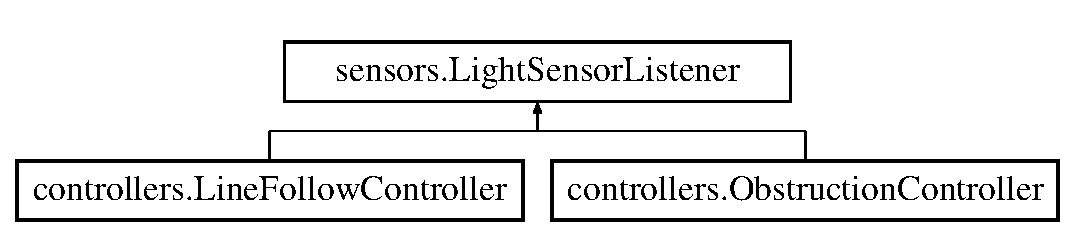
\includegraphics[height=2.000000cm]{interfacesensors_1_1_light_sensor_listener}
\end{center}
\end{figure}
\subsection*{Public Member Functions}
\begin{DoxyCompactItemize}
\item 
void \hyperlink{interfacesensors_1_1_light_sensor_listener_ad454a7e5082bc820b4cc27cf173a111a}{light\-Sensor\-Changed} (\hyperlink{enumsensors_1_1_position}{Position} position, \hyperlink{interfacesensors_1_1_updating_sensor}{Updating\-Sensor} updatingsensor, float old\-Value, float new\-Value)
\end{DoxyCompactItemize}


\subsection{Detailed Description}
This is the light sensor listener interface

\begin{DoxyAuthor}{Author}
Robert Bezem \href{mailto:robert.bezem@student.hu.nl}{\tt robert.\-bezem@student.\-hu.\-nl} 
\end{DoxyAuthor}
\begin{DoxyVersion}{Version}
1.\-0 
\end{DoxyVersion}
\begin{DoxySince}{Since}
01-\/04-\/2014 
\end{DoxySince}


\subsection{Member Function Documentation}
\hypertarget{interfacesensors_1_1_light_sensor_listener_ad454a7e5082bc820b4cc27cf173a111a}{\index{sensors\-::\-Light\-Sensor\-Listener@{sensors\-::\-Light\-Sensor\-Listener}!light\-Sensor\-Changed@{light\-Sensor\-Changed}}
\index{light\-Sensor\-Changed@{light\-Sensor\-Changed}!sensors::LightSensorListener@{sensors\-::\-Light\-Sensor\-Listener}}
\subsubsection[{light\-Sensor\-Changed}]{\setlength{\rightskip}{0pt plus 5cm}void sensors.\-Light\-Sensor\-Listener.\-light\-Sensor\-Changed (
\begin{DoxyParamCaption}
\item[{{\bf Position}}]{position, }
\item[{{\bf Updating\-Sensor}}]{updatingsensor, }
\item[{float}]{old\-Value, }
\item[{float}]{new\-Value}
\end{DoxyParamCaption}
)}}\label{interfacesensors_1_1_light_sensor_listener_ad454a7e5082bc820b4cc27cf173a111a}
When this class is being implemented, this class will be called upon when one of the light sensors' state changes.


\begin{DoxyParams}{Parameters}
{\em position} & the position of the sensor used \\
\hline
{\em updatingsensor} & the sensor that is been updated \\
\hline
{\em old\-Value} & the value before the change \\
\hline
{\em new\-Value} & the value after the change \\
\hline
\end{DoxyParams}


Implemented in \hyperlink{classcontrollers_1_1_line_follow_controller_a673cf765cff30bc14f9bfd8eb54dc6dd}{controllers.\-Line\-Follow\-Controller}, and \hyperlink{classcontrollers_1_1_obstruction_controller_ae8627b8e53bd16dcefeb5b84dfc55ee5}{controllers.\-Obstruction\-Controller}.



The documentation for this interface was generated from the following file\-:\begin{DoxyCompactItemize}
\item 
C\-:/\-Users/hp/git/the\-End/\-Eind\-Project/src/sensors/\hyperlink{_light_sensor_listener_8java}{Light\-Sensor\-Listener.\-java}\end{DoxyCompactItemize}

\hypertarget{classcontrollers_1_1_line_follow_controller}{\section{controllers.\-Line\-Follow\-Controller Class Reference}
\label{classcontrollers_1_1_line_follow_controller}\index{controllers.\-Line\-Follow\-Controller@{controllers.\-Line\-Follow\-Controller}}
}
Inheritance diagram for controllers.\-Line\-Follow\-Controller\-:\begin{figure}[H]
\begin{center}
\leavevmode
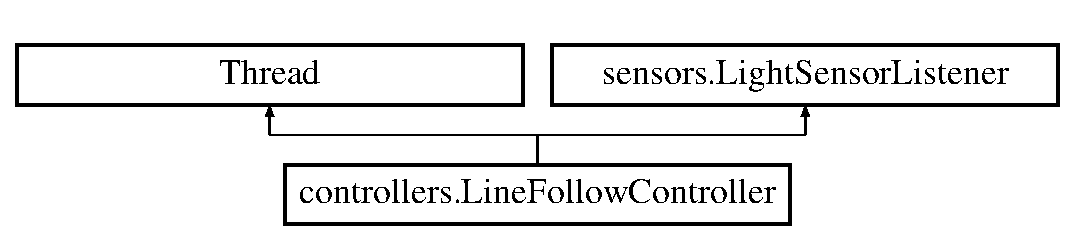
\includegraphics[height=2.000000cm]{classcontrollers_1_1_line_follow_controller}
\end{center}
\end{figure}
\subsection*{Public Member Functions}
\begin{DoxyCompactItemize}
\item 
\hyperlink{classcontrollers_1_1_line_follow_controller_a3d348192dadb4523ea57a9165720a01d}{Line\-Follow\-Controller} (\hyperlink{classsensors_1_1_my_color_sensor}{My\-Color\-Sensor} cs, \hyperlink{classsensors_1_1_my_light_sensor}{My\-Light\-Sensor} ls, \hyperlink{classgui_1_1_g_u_i}{G\-U\-I} gui)
\item 
void \hyperlink{classcontrollers_1_1_line_follow_controller_ab0d8c9fa9e91633438c1e4ae778017fa}{run} ()
\item 
void \hyperlink{classcontrollers_1_1_line_follow_controller_afeee12743ec4cedb303c6b6cd72489bd}{set\-Active} (boolean incoming\-Value)
\item 
void \hyperlink{classcontrollers_1_1_line_follow_controller_a673cf765cff30bc14f9bfd8eb54dc6dd}{light\-Sensor\-Changed} (\hyperlink{enumsensors_1_1_position}{Position} position, \hyperlink{interfacesensors_1_1_updating_sensor}{Updating\-Sensor} updatingsensor, float old\-Value, float new\-Value)
\end{DoxyCompactItemize}
\subsection*{Static Public Member Functions}
\begin{DoxyCompactItemize}
\item 
static void \hyperlink{classcontrollers_1_1_line_follow_controller_a304089767b35529b1aa8e0d6c9355109}{pause\-Line\-Follower} ()
\item 
static void \hyperlink{classcontrollers_1_1_line_follow_controller_aefc55f5d77bcc8a1ac339e08adc5bccb}{continue\-Line\-Follower} ()
\end{DoxyCompactItemize}


\subsection{Detailed Description}
This class will guide a Lego N\-X\-T Robot via a black trail on a white surface.

\begin{DoxyAuthor}{Author}
Pim van Hespen \href{mailto:PimvanHespen@gmail.com}{\tt Pimvan\-Hespen@gmail.\-com} 

Jacob Visser \href{mailto:Jacob.Visser@student.hu.nl}{\tt Jacob.\-Visser@student.\-hu.\-nl} 

Robert Bezem \href{mailto:Robert.Bezem@student.hu.nl}{\tt Robert.\-Bezem@student.\-hu.\-nl} 
\end{DoxyAuthor}
\begin{DoxyVersion}{Version}
1.\-5 
\end{DoxyVersion}
\begin{DoxySince}{Since}
04-\/04-\/2014 
\end{DoxySince}


\subsection{Constructor \& Destructor Documentation}
\hypertarget{classcontrollers_1_1_line_follow_controller_a3d348192dadb4523ea57a9165720a01d}{\index{controllers\-::\-Line\-Follow\-Controller@{controllers\-::\-Line\-Follow\-Controller}!Line\-Follow\-Controller@{Line\-Follow\-Controller}}
\index{Line\-Follow\-Controller@{Line\-Follow\-Controller}!controllers::LineFollowController@{controllers\-::\-Line\-Follow\-Controller}}
\subsubsection[{Line\-Follow\-Controller}]{\setlength{\rightskip}{0pt plus 5cm}controllers.\-Line\-Follow\-Controller.\-Line\-Follow\-Controller (
\begin{DoxyParamCaption}
\item[{{\bf My\-Color\-Sensor}}]{cs, }
\item[{{\bf My\-Light\-Sensor}}]{ls, }
\item[{{\bf G\-U\-I}}]{gui}
\end{DoxyParamCaption}
)}}\label{classcontrollers_1_1_line_follow_controller_a3d348192dadb4523ea57a9165720a01d}


\subsection{Member Function Documentation}
\hypertarget{classcontrollers_1_1_line_follow_controller_aefc55f5d77bcc8a1ac339e08adc5bccb}{\index{controllers\-::\-Line\-Follow\-Controller@{controllers\-::\-Line\-Follow\-Controller}!continue\-Line\-Follower@{continue\-Line\-Follower}}
\index{continue\-Line\-Follower@{continue\-Line\-Follower}!controllers::LineFollowController@{controllers\-::\-Line\-Follow\-Controller}}
\subsubsection[{continue\-Line\-Follower}]{\setlength{\rightskip}{0pt plus 5cm}static void controllers.\-Line\-Follow\-Controller.\-continue\-Line\-Follower (
\begin{DoxyParamCaption}
{}
\end{DoxyParamCaption}
)\hspace{0.3cm}{\ttfamily [static]}}}\label{classcontrollers_1_1_line_follow_controller_aefc55f5d77bcc8a1ac339e08adc5bccb}
\hypertarget{classcontrollers_1_1_line_follow_controller_a673cf765cff30bc14f9bfd8eb54dc6dd}{\index{controllers\-::\-Line\-Follow\-Controller@{controllers\-::\-Line\-Follow\-Controller}!light\-Sensor\-Changed@{light\-Sensor\-Changed}}
\index{light\-Sensor\-Changed@{light\-Sensor\-Changed}!controllers::LineFollowController@{controllers\-::\-Line\-Follow\-Controller}}
\subsubsection[{light\-Sensor\-Changed}]{\setlength{\rightskip}{0pt plus 5cm}void controllers.\-Line\-Follow\-Controller.\-light\-Sensor\-Changed (
\begin{DoxyParamCaption}
\item[{{\bf Position}}]{position, }
\item[{{\bf Updating\-Sensor}}]{updatingsensor, }
\item[{float}]{old\-Value, }
\item[{float}]{new\-Value}
\end{DoxyParamCaption}
)}}\label{classcontrollers_1_1_line_follow_controller_a673cf765cff30bc14f9bfd8eb54dc6dd}
\begin{DoxySeeAlso}{See Also}
\hyperlink{interfacesensors_1_1_light_sensor_listener_ad454a7e5082bc820b4cc27cf173a111a}{sensors.\-Light\-Sensor\-Listener\-::light\-Sensor\-Changed}(sensors.\-Sensor\-Position, \hyperlink{interfacesensors_1_1_updating_sensor}{sensors.\-Updating\-Sensor}, float, float) 
\end{DoxySeeAlso}


Implements \hyperlink{interfacesensors_1_1_light_sensor_listener_ad454a7e5082bc820b4cc27cf173a111a}{sensors.\-Light\-Sensor\-Listener}.

\hypertarget{classcontrollers_1_1_line_follow_controller_a304089767b35529b1aa8e0d6c9355109}{\index{controllers\-::\-Line\-Follow\-Controller@{controllers\-::\-Line\-Follow\-Controller}!pause\-Line\-Follower@{pause\-Line\-Follower}}
\index{pause\-Line\-Follower@{pause\-Line\-Follower}!controllers::LineFollowController@{controllers\-::\-Line\-Follow\-Controller}}
\subsubsection[{pause\-Line\-Follower}]{\setlength{\rightskip}{0pt plus 5cm}static void controllers.\-Line\-Follow\-Controller.\-pause\-Line\-Follower (
\begin{DoxyParamCaption}
{}
\end{DoxyParamCaption}
)\hspace{0.3cm}{\ttfamily [static]}}}\label{classcontrollers_1_1_line_follow_controller_a304089767b35529b1aa8e0d6c9355109}
\hypertarget{classcontrollers_1_1_line_follow_controller_ab0d8c9fa9e91633438c1e4ae778017fa}{\index{controllers\-::\-Line\-Follow\-Controller@{controllers\-::\-Line\-Follow\-Controller}!run@{run}}
\index{run@{run}!controllers::LineFollowController@{controllers\-::\-Line\-Follow\-Controller}}
\subsubsection[{run}]{\setlength{\rightskip}{0pt plus 5cm}void controllers.\-Line\-Follow\-Controller.\-run (
\begin{DoxyParamCaption}
{}
\end{DoxyParamCaption}
)}}\label{classcontrollers_1_1_line_follow_controller_ab0d8c9fa9e91633438c1e4ae778017fa}
\hypertarget{classcontrollers_1_1_line_follow_controller_afeee12743ec4cedb303c6b6cd72489bd}{\index{controllers\-::\-Line\-Follow\-Controller@{controllers\-::\-Line\-Follow\-Controller}!set\-Active@{set\-Active}}
\index{set\-Active@{set\-Active}!controllers::LineFollowController@{controllers\-::\-Line\-Follow\-Controller}}
\subsubsection[{set\-Active}]{\setlength{\rightskip}{0pt plus 5cm}void controllers.\-Line\-Follow\-Controller.\-set\-Active (
\begin{DoxyParamCaption}
\item[{boolean}]{incoming\-Value}
\end{DoxyParamCaption}
)}}\label{classcontrollers_1_1_line_follow_controller_afeee12743ec4cedb303c6b6cd72489bd}
This is the setter for boolean 'active'.


\begin{DoxyParams}{Parameters}
{\em incoming\-Value} & the value to set active to. \\
\hline
\end{DoxyParams}


The documentation for this class was generated from the following file\-:\begin{DoxyCompactItemize}
\item 
C\-:/\-Users/hp/git/the\-End/\-Eind\-Project/src/controllers/\hyperlink{_line_follow_controller_8java}{Line\-Follow\-Controller.\-java}\end{DoxyCompactItemize}

\hypertarget{classnxt_1_1_main}{\section{nxt.\-Main Class Reference}
\label{classnxt_1_1_main}\index{nxt.\-Main@{nxt.\-Main}}
}
\subsection*{Static Public Member Functions}
\begin{DoxyCompactItemize}
\item 
static void \hyperlink{classnxt_1_1_main_a73f9a37e6e61b9174cc8cac8fc83b46d}{main} (String\mbox{[}$\,$\mbox{]} args)
\end{DoxyCompactItemize}


\subsection{Detailed Description}
This class starts all required controllers to control the robot.

\begin{DoxyAuthor}{Author}
Jacob Visser \href{mailto:Jacob.Visser@student.hu.nl}{\tt Jacob.\-Visser@student.\-hu.\-nl} 

Pim van Hespen \href{mailto:PimvanHespen@gmail.com}{\tt Pimvan\-Hespen@gmail.\-com} 

Robert Bezem \href{mailto:Robert.Bezem@student.hu.nl}{\tt Robert.\-Bezem@student.\-hu.\-nl} 
\end{DoxyAuthor}
\begin{DoxySince}{Since}
01-\/04-\/2014 
\end{DoxySince}
\begin{DoxyVersion}{Version}
2.\-0 
\end{DoxyVersion}


\subsection{Member Function Documentation}
\hypertarget{classnxt_1_1_main_a73f9a37e6e61b9174cc8cac8fc83b46d}{\index{nxt\-::\-Main@{nxt\-::\-Main}!main@{main}}
\index{main@{main}!nxt::Main@{nxt\-::\-Main}}
\subsubsection[{main}]{\setlength{\rightskip}{0pt plus 5cm}static void nxt.\-Main.\-main (
\begin{DoxyParamCaption}
\item[{String\mbox{[}$\,$\mbox{]}}]{args}
\end{DoxyParamCaption}
)\hspace{0.3cm}{\ttfamily [static]}}}\label{classnxt_1_1_main_a73f9a37e6e61b9174cc8cac8fc83b46d}
This method defines all sensors and creates the controllers


\begin{DoxyParams}{Parameters}
{\em args} & incoming arguments from outside the code \\
\hline
\end{DoxyParams}


The documentation for this class was generated from the following file\-:\begin{DoxyCompactItemize}
\item 
C\-:/\-Users/hp/git/the\-End/\-Eind\-Project/src/nxt/\hyperlink{_main_8java}{Main.\-java}\end{DoxyCompactItemize}

\hypertarget{classmotors_1_1_motor_controller}{\section{motors.\-Motor\-Controller Class Reference}
\label{classmotors_1_1_motor_controller}\index{motors.\-Motor\-Controller@{motors.\-Motor\-Controller}}
}
\subsection*{Static Public Member Functions}
\begin{DoxyCompactItemize}
\item 
static void \hyperlink{classmotors_1_1_motor_controller_a27a982c9114f012616ede0c49dd26880}{drive\-Arc} (float turn\-Radius)
\item 
static void \hyperlink{classmotors_1_1_motor_controller_a7010c7902838c03055daf3176c093bc4}{drive\-Forward} ()
\item 
static void \hyperlink{classmotors_1_1_motor_controller_ab4b6b46388aab6adb952e222d2d53f31}{stop} ()
\item 
static void \hyperlink{classmotors_1_1_motor_controller_af036b71f8836e9fcf32e0c7590b3e3e0}{drive\-Backwards} ()
\item 
static void \hyperlink{classmotors_1_1_motor_controller_ac200a0e610365d4d7f501d760e0fb5dc}{drive\-Distance} (float distance)
\item 
static boolean \hyperlink{classmotors_1_1_motor_controller_ab171d0d83a4ddcc87062b2c20721928f}{moving} ()
\item 
static void \hyperlink{classmotors_1_1_motor_controller_a6d617fcbcc35b8067bf10cdaafc94406}{drive\-Arc} (float turn\-Radius, boolean immediate\-Return)
\item 
static void \hyperlink{classmotors_1_1_motor_controller_ab99c3b5ae070cbe7034e8a49db9a59ef}{drive\-Arc} (int radius, int degrees, boolean immmediate\-Return)
\item 
static void \hyperlink{classmotors_1_1_motor_controller_a30bba3cbbbfe8fe774b21a58fba75e3b}{rotate} (int degrees, boolean immediate\-Return)
\item 
static void \hyperlink{classmotors_1_1_motor_controller_a129bd9d50a6d50c7d69e76415f798f17}{set\-Rotate\-Speed} (float degrees)
\item 
static void \hyperlink{classmotors_1_1_motor_controller_af3781222ae2e4fe3df581b14d79f3a40}{set\-Travel\-Speed} (float speed)
\item 
static void \hyperlink{classmotors_1_1_motor_controller_a13919e49cdf9aa70573a4beef99cda3c}{set\-Individiual\-Traval\-Speed} (int left\-Motor\-Speed, int right\-Motor\-Speed)
\item 
static void \hyperlink{classmotors_1_1_motor_controller_a5faee69ef82085ae5c1bf9e8f786387c}{set\-Left\-Motor\-Speed} (int speed)
\item 
static void \hyperlink{classmotors_1_1_motor_controller_a9a49fc2ea035ba507c97a8f20bead2f0}{set\-Right\-Motor\-Speed} (int speed)
\item 
static double \hyperlink{classmotors_1_1_motor_controller_a1cf8566e8b8fca27a1ac16aab1b93c2a}{get\-Rotatepeed} ()
\item 
static double \hyperlink{classmotors_1_1_motor_controller_a84c24ed7d98b6e818506182321402d9f}{get\-Travel\-Speed} ()
\end{DoxyCompactItemize}


\subsection{Detailed Description}
This class allows other classes to steer the motor

\begin{DoxyAuthor}{Author}
Robert Bezem \href{mailto:robert.bezem@student.hu.nl}{\tt robert.\-bezem@student.\-hu.\-nl} 

Jacob Visser \href{mailto:jacob.visser@student.hu.nl}{\tt jacob.\-visser@student.\-hu.\-nl} 

Pim van Hespen \href{mailto:pimvanhespen@gmail.com}{\tt pimvanhespen@gmail.\-com} 
\end{DoxyAuthor}
\begin{DoxyVersion}{Version}
1.\-5 
\end{DoxyVersion}
\begin{DoxySince}{Since}
01-\/04-\/2014 
\end{DoxySince}


\subsection{Member Function Documentation}
\hypertarget{classmotors_1_1_motor_controller_a27a982c9114f012616ede0c49dd26880}{\index{motors\-::\-Motor\-Controller@{motors\-::\-Motor\-Controller}!drive\-Arc@{drive\-Arc}}
\index{drive\-Arc@{drive\-Arc}!motors::MotorController@{motors\-::\-Motor\-Controller}}
\subsubsection[{drive\-Arc}]{\setlength{\rightskip}{0pt plus 5cm}static void motors.\-Motor\-Controller.\-drive\-Arc (
\begin{DoxyParamCaption}
\item[{float}]{turn\-Radius}
\end{DoxyParamCaption}
)\hspace{0.3cm}{\ttfamily [static]}}}\label{classmotors_1_1_motor_controller_a27a982c9114f012616ede0c49dd26880}
Will make the robot drive arc with the given radius. Stops when motor is stopped


\begin{DoxyParams}{Parameters}
{\em turn\-Radius} & radius in millimeter \\
\hline
\end{DoxyParams}
\hypertarget{classmotors_1_1_motor_controller_a6d617fcbcc35b8067bf10cdaafc94406}{\index{motors\-::\-Motor\-Controller@{motors\-::\-Motor\-Controller}!drive\-Arc@{drive\-Arc}}
\index{drive\-Arc@{drive\-Arc}!motors::MotorController@{motors\-::\-Motor\-Controller}}
\subsubsection[{drive\-Arc}]{\setlength{\rightskip}{0pt plus 5cm}static void motors.\-Motor\-Controller.\-drive\-Arc (
\begin{DoxyParamCaption}
\item[{float}]{turn\-Radius, }
\item[{boolean}]{immediate\-Return}
\end{DoxyParamCaption}
)\hspace{0.3cm}{\ttfamily [static]}}}\label{classmotors_1_1_motor_controller_a6d617fcbcc35b8067bf10cdaafc94406}
Makes the robot drive a circle with the given radius 'turn\-Radius'


\begin{DoxyParams}{Parameters}
{\em turn\-Radius} & radius in millimeters \\
\hline
{\em immediate\-Return} & if true, immediately returns to the next line of code while executing the arc \\
\hline
\end{DoxyParams}
\hypertarget{classmotors_1_1_motor_controller_ab99c3b5ae070cbe7034e8a49db9a59ef}{\index{motors\-::\-Motor\-Controller@{motors\-::\-Motor\-Controller}!drive\-Arc@{drive\-Arc}}
\index{drive\-Arc@{drive\-Arc}!motors::MotorController@{motors\-::\-Motor\-Controller}}
\subsubsection[{drive\-Arc}]{\setlength{\rightskip}{0pt plus 5cm}static void motors.\-Motor\-Controller.\-drive\-Arc (
\begin{DoxyParamCaption}
\item[{int}]{radius, }
\item[{int}]{degrees, }
\item[{boolean}]{immmediate\-Return}
\end{DoxyParamCaption}
)\hspace{0.3cm}{\ttfamily [static]}}}\label{classmotors_1_1_motor_controller_ab99c3b5ae070cbe7034e8a49db9a59ef}

\begin{DoxyParams}{Parameters}
{\em radius} & of the arc in millimeters \\
\hline
{\em degrees} & of the arc to drive \\
\hline
{\em immmediate\-Return} & if true, immediately returns to the next line of code while executing the arc \\
\hline
\end{DoxyParams}
\hypertarget{classmotors_1_1_motor_controller_af036b71f8836e9fcf32e0c7590b3e3e0}{\index{motors\-::\-Motor\-Controller@{motors\-::\-Motor\-Controller}!drive\-Backwards@{drive\-Backwards}}
\index{drive\-Backwards@{drive\-Backwards}!motors::MotorController@{motors\-::\-Motor\-Controller}}
\subsubsection[{drive\-Backwards}]{\setlength{\rightskip}{0pt plus 5cm}static void motors.\-Motor\-Controller.\-drive\-Backwards (
\begin{DoxyParamCaption}
{}
\end{DoxyParamCaption}
)\hspace{0.3cm}{\ttfamily [static]}}}\label{classmotors_1_1_motor_controller_af036b71f8836e9fcf32e0c7590b3e3e0}
Will move the robot backwards until stopped \hypertarget{classmotors_1_1_motor_controller_ac200a0e610365d4d7f501d760e0fb5dc}{\index{motors\-::\-Motor\-Controller@{motors\-::\-Motor\-Controller}!drive\-Distance@{drive\-Distance}}
\index{drive\-Distance@{drive\-Distance}!motors::MotorController@{motors\-::\-Motor\-Controller}}
\subsubsection[{drive\-Distance}]{\setlength{\rightskip}{0pt plus 5cm}static void motors.\-Motor\-Controller.\-drive\-Distance (
\begin{DoxyParamCaption}
\item[{float}]{distance}
\end{DoxyParamCaption}
)\hspace{0.3cm}{\ttfamily [static]}}}\label{classmotors_1_1_motor_controller_ac200a0e610365d4d7f501d760e0fb5dc}
Moves the robot for a set amount


\begin{DoxyParams}{Parameters}
{\em distance} & in millimeters \\
\hline
\end{DoxyParams}
\hypertarget{classmotors_1_1_motor_controller_a7010c7902838c03055daf3176c093bc4}{\index{motors\-::\-Motor\-Controller@{motors\-::\-Motor\-Controller}!drive\-Forward@{drive\-Forward}}
\index{drive\-Forward@{drive\-Forward}!motors::MotorController@{motors\-::\-Motor\-Controller}}
\subsubsection[{drive\-Forward}]{\setlength{\rightskip}{0pt plus 5cm}static void motors.\-Motor\-Controller.\-drive\-Forward (
\begin{DoxyParamCaption}
{}
\end{DoxyParamCaption}
)\hspace{0.3cm}{\ttfamily [static]}}}\label{classmotors_1_1_motor_controller_a7010c7902838c03055daf3176c093bc4}
Will move the robot forward until canceled \hypertarget{classmotors_1_1_motor_controller_a1cf8566e8b8fca27a1ac16aab1b93c2a}{\index{motors\-::\-Motor\-Controller@{motors\-::\-Motor\-Controller}!get\-Rotatepeed@{get\-Rotatepeed}}
\index{get\-Rotatepeed@{get\-Rotatepeed}!motors::MotorController@{motors\-::\-Motor\-Controller}}
\subsubsection[{get\-Rotatepeed}]{\setlength{\rightskip}{0pt plus 5cm}static double motors.\-Motor\-Controller.\-get\-Rotatepeed (
\begin{DoxyParamCaption}
{}
\end{DoxyParamCaption}
)\hspace{0.3cm}{\ttfamily [static]}}}\label{classmotors_1_1_motor_controller_a1cf8566e8b8fca27a1ac16aab1b93c2a}
\hypertarget{classmotors_1_1_motor_controller_a84c24ed7d98b6e818506182321402d9f}{\index{motors\-::\-Motor\-Controller@{motors\-::\-Motor\-Controller}!get\-Travel\-Speed@{get\-Travel\-Speed}}
\index{get\-Travel\-Speed@{get\-Travel\-Speed}!motors::MotorController@{motors\-::\-Motor\-Controller}}
\subsubsection[{get\-Travel\-Speed}]{\setlength{\rightskip}{0pt plus 5cm}static double motors.\-Motor\-Controller.\-get\-Travel\-Speed (
\begin{DoxyParamCaption}
{}
\end{DoxyParamCaption}
)\hspace{0.3cm}{\ttfamily [static]}}}\label{classmotors_1_1_motor_controller_a84c24ed7d98b6e818506182321402d9f}
\hypertarget{classmotors_1_1_motor_controller_ab171d0d83a4ddcc87062b2c20721928f}{\index{motors\-::\-Motor\-Controller@{motors\-::\-Motor\-Controller}!moving@{moving}}
\index{moving@{moving}!motors::MotorController@{motors\-::\-Motor\-Controller}}
\subsubsection[{moving}]{\setlength{\rightskip}{0pt plus 5cm}static boolean motors.\-Motor\-Controller.\-moving (
\begin{DoxyParamCaption}
{}
\end{DoxyParamCaption}
)\hspace{0.3cm}{\ttfamily [static]}}}\label{classmotors_1_1_motor_controller_ab171d0d83a4ddcc87062b2c20721928f}
Tells if the robot is moving (true) or isn't (false)

\begin{DoxyReturn}{Returns}
if the robot is moving 
\end{DoxyReturn}
\hypertarget{classmotors_1_1_motor_controller_a30bba3cbbbfe8fe774b21a58fba75e3b}{\index{motors\-::\-Motor\-Controller@{motors\-::\-Motor\-Controller}!rotate@{rotate}}
\index{rotate@{rotate}!motors::MotorController@{motors\-::\-Motor\-Controller}}
\subsubsection[{rotate}]{\setlength{\rightskip}{0pt plus 5cm}static void motors.\-Motor\-Controller.\-rotate (
\begin{DoxyParamCaption}
\item[{int}]{degrees, }
\item[{boolean}]{immediate\-Return}
\end{DoxyParamCaption}
)\hspace{0.3cm}{\ttfamily [static]}}}\label{classmotors_1_1_motor_controller_a30bba3cbbbfe8fe774b21a58fba75e3b}

\begin{DoxyParams}{Parameters}
{\em degrees} & to turn \\
\hline
{\em immmediate\-Return} & if true, immediately returns to the next line of code while executing the rotation \\
\hline
\end{DoxyParams}
\hypertarget{classmotors_1_1_motor_controller_a13919e49cdf9aa70573a4beef99cda3c}{\index{motors\-::\-Motor\-Controller@{motors\-::\-Motor\-Controller}!set\-Individiual\-Traval\-Speed@{set\-Individiual\-Traval\-Speed}}
\index{set\-Individiual\-Traval\-Speed@{set\-Individiual\-Traval\-Speed}!motors::MotorController@{motors\-::\-Motor\-Controller}}
\subsubsection[{set\-Individiual\-Traval\-Speed}]{\setlength{\rightskip}{0pt plus 5cm}static void motors.\-Motor\-Controller.\-set\-Individiual\-Traval\-Speed (
\begin{DoxyParamCaption}
\item[{int}]{left\-Motor\-Speed, }
\item[{int}]{right\-Motor\-Speed}
\end{DoxyParamCaption}
)\hspace{0.3cm}{\ttfamily [static]}}}\label{classmotors_1_1_motor_controller_a13919e49cdf9aa70573a4beef99cda3c}
set individual motor speeds


\begin{DoxyParams}{Parameters}
{\em left\-Motor\-Speed} & in degrees per second \\
\hline
{\em right\-Motor\-Speed} & in degrees per second \\
\hline
\end{DoxyParams}
\hypertarget{classmotors_1_1_motor_controller_a5faee69ef82085ae5c1bf9e8f786387c}{\index{motors\-::\-Motor\-Controller@{motors\-::\-Motor\-Controller}!set\-Left\-Motor\-Speed@{set\-Left\-Motor\-Speed}}
\index{set\-Left\-Motor\-Speed@{set\-Left\-Motor\-Speed}!motors::MotorController@{motors\-::\-Motor\-Controller}}
\subsubsection[{set\-Left\-Motor\-Speed}]{\setlength{\rightskip}{0pt plus 5cm}static void motors.\-Motor\-Controller.\-set\-Left\-Motor\-Speed (
\begin{DoxyParamCaption}
\item[{int}]{speed}
\end{DoxyParamCaption}
)\hspace{0.3cm}{\ttfamily [static]}}}\label{classmotors_1_1_motor_controller_a5faee69ef82085ae5c1bf9e8f786387c}
sets speed for the left motor


\begin{DoxyParams}{Parameters}
{\em speed} & in degrees per second \\
\hline
\end{DoxyParams}
\hypertarget{classmotors_1_1_motor_controller_a9a49fc2ea035ba507c97a8f20bead2f0}{\index{motors\-::\-Motor\-Controller@{motors\-::\-Motor\-Controller}!set\-Right\-Motor\-Speed@{set\-Right\-Motor\-Speed}}
\index{set\-Right\-Motor\-Speed@{set\-Right\-Motor\-Speed}!motors::MotorController@{motors\-::\-Motor\-Controller}}
\subsubsection[{set\-Right\-Motor\-Speed}]{\setlength{\rightskip}{0pt plus 5cm}static void motors.\-Motor\-Controller.\-set\-Right\-Motor\-Speed (
\begin{DoxyParamCaption}
\item[{int}]{speed}
\end{DoxyParamCaption}
)\hspace{0.3cm}{\ttfamily [static]}}}\label{classmotors_1_1_motor_controller_a9a49fc2ea035ba507c97a8f20bead2f0}
sets speed for the right motor


\begin{DoxyParams}{Parameters}
{\em speed} & in degrees per second \\
\hline
\end{DoxyParams}
\hypertarget{classmotors_1_1_motor_controller_a129bd9d50a6d50c7d69e76415f798f17}{\index{motors\-::\-Motor\-Controller@{motors\-::\-Motor\-Controller}!set\-Rotate\-Speed@{set\-Rotate\-Speed}}
\index{set\-Rotate\-Speed@{set\-Rotate\-Speed}!motors::MotorController@{motors\-::\-Motor\-Controller}}
\subsubsection[{set\-Rotate\-Speed}]{\setlength{\rightskip}{0pt plus 5cm}static void motors.\-Motor\-Controller.\-set\-Rotate\-Speed (
\begin{DoxyParamCaption}
\item[{float}]{degrees}
\end{DoxyParamCaption}
)\hspace{0.3cm}{\ttfamily [static]}}}\label{classmotors_1_1_motor_controller_a129bd9d50a6d50c7d69e76415f798f17}
set the degrees to turn per second


\begin{DoxyParams}{Parameters}
{\em degrees} & per second \\
\hline
\end{DoxyParams}
\hypertarget{classmotors_1_1_motor_controller_af3781222ae2e4fe3df581b14d79f3a40}{\index{motors\-::\-Motor\-Controller@{motors\-::\-Motor\-Controller}!set\-Travel\-Speed@{set\-Travel\-Speed}}
\index{set\-Travel\-Speed@{set\-Travel\-Speed}!motors::MotorController@{motors\-::\-Motor\-Controller}}
\subsubsection[{set\-Travel\-Speed}]{\setlength{\rightskip}{0pt plus 5cm}static void motors.\-Motor\-Controller.\-set\-Travel\-Speed (
\begin{DoxyParamCaption}
\item[{float}]{speed}
\end{DoxyParamCaption}
)\hspace{0.3cm}{\ttfamily [static]}}}\label{classmotors_1_1_motor_controller_af3781222ae2e4fe3df581b14d79f3a40}
sets the travel\-Speed


\begin{DoxyParams}{Parameters}
{\em speed} & in wheel diameter/units per second \\
\hline
\end{DoxyParams}
\hypertarget{classmotors_1_1_motor_controller_ab4b6b46388aab6adb952e222d2d53f31}{\index{motors\-::\-Motor\-Controller@{motors\-::\-Motor\-Controller}!stop@{stop}}
\index{stop@{stop}!motors::MotorController@{motors\-::\-Motor\-Controller}}
\subsubsection[{stop}]{\setlength{\rightskip}{0pt plus 5cm}static void motors.\-Motor\-Controller.\-stop (
\begin{DoxyParamCaption}
{}
\end{DoxyParamCaption}
)\hspace{0.3cm}{\ttfamily [static]}}}\label{classmotors_1_1_motor_controller_ab4b6b46388aab6adb952e222d2d53f31}
stops all movement. 

The documentation for this class was generated from the following file\-:\begin{DoxyCompactItemize}
\item 
C\-:/\-Users/hp/git/the\-End/\-Eind\-Project/src/motors/\hyperlink{_motor_controller_8java}{Motor\-Controller.\-java}\end{DoxyCompactItemize}

\hypertarget{classsensors_1_1_my_color_sensor}{\section{sensors.\-My\-Color\-Sensor Class Reference}
\label{classsensors_1_1_my_color_sensor}\index{sensors.\-My\-Color\-Sensor@{sensors.\-My\-Color\-Sensor}}
}
Inheritance diagram for sensors.\-My\-Color\-Sensor\-:\begin{figure}[H]
\begin{center}
\leavevmode
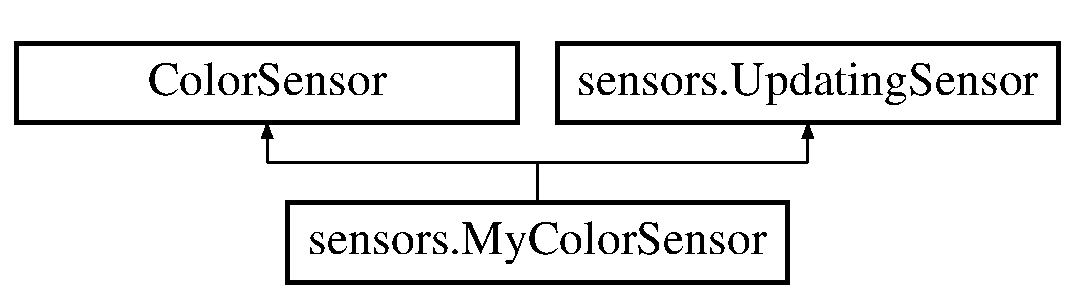
\includegraphics[height=2.000000cm]{classsensors_1_1_my_color_sensor}
\end{center}
\end{figure}
\subsection*{Public Member Functions}
\begin{DoxyCompactItemize}
\item 
\hyperlink{classsensors_1_1_my_color_sensor_a9058deb72ccfa0f38def0b10e971be76}{My\-Color\-Sensor} (Sensor\-Port sensorport, \hyperlink{enumsensors_1_1_position}{Position} position)
\item 
void \hyperlink{classsensors_1_1_my_color_sensor_a17324aa0de8fa9ab45bb2c1450e0119a}{update\-State} ()
\item 
void \hyperlink{classsensors_1_1_my_color_sensor_aed2d2c661c0d980695bbfc4bb21a9f2f}{add\-Listener} (\hyperlink{interfacesensors_1_1_light_sensor_listener}{Light\-Sensor\-Listener} listener)
\item 
void \hyperlink{classsensors_1_1_my_color_sensor_a2cc8382833eeb064afde388d243efe08}{delete\-Listener} (\hyperlink{interfacesensors_1_1_light_sensor_listener}{Light\-Sensor\-Listener} listener)
\item 
int \hyperlink{classsensors_1_1_my_color_sensor_aa61cdd8b3ed7ab6355a79173949d816d}{get\-Light\-Value} ()
\item 
int \hyperlink{classsensors_1_1_my_color_sensor_a33a47875addf7ccd00aa6fa63e5a9219}{get\-Low} ()
\item 
int \hyperlink{classsensors_1_1_my_color_sensor_aa988dadec2aafa7fcf6636b12244ef1a}{get\-High} ()
\item 
void \hyperlink{classsensors_1_1_my_color_sensor_a1dc583efb6f3f4e978af6d52c8a702b0}{set\-High} (int value)
\item 
void \hyperlink{classsensors_1_1_my_color_sensor_a8929a9791cbdc348082600c01a63f17a}{set\-Low} (int value)
\item 
\hyperlink{enumsensors_1_1_sensor_type}{Sensor\-Type} \hyperlink{classsensors_1_1_my_color_sensor_a62eaf9476cb88ab8e77f720e7953c6cd}{get\-Sensor\-Type} ()
\end{DoxyCompactItemize}


\subsection{Detailed Description}
\begin{DoxyAuthor}{Author}
Robert Bezem \href{mailto:robert.bezem@student.hu.nl}{\tt robert.\-bezem@student.\-hu.\-nl} 
\end{DoxyAuthor}
\begin{DoxyVersion}{Version}
1.\-0 
\end{DoxyVersion}
\begin{DoxySince}{Since}
01-\/04-\/2014 
\end{DoxySince}


\subsection{Constructor \& Destructor Documentation}
\hypertarget{classsensors_1_1_my_color_sensor_a9058deb72ccfa0f38def0b10e971be76}{\index{sensors\-::\-My\-Color\-Sensor@{sensors\-::\-My\-Color\-Sensor}!My\-Color\-Sensor@{My\-Color\-Sensor}}
\index{My\-Color\-Sensor@{My\-Color\-Sensor}!sensors::MyColorSensor@{sensors\-::\-My\-Color\-Sensor}}
\subsubsection[{My\-Color\-Sensor}]{\setlength{\rightskip}{0pt plus 5cm}sensors.\-My\-Color\-Sensor.\-My\-Color\-Sensor (
\begin{DoxyParamCaption}
\item[{Sensor\-Port}]{sensorport, }
\item[{{\bf Position}}]{position}
\end{DoxyParamCaption}
)}}\label{classsensors_1_1_my_color_sensor_a9058deb72ccfa0f38def0b10e971be76}
The constructor for the \hyperlink{classsensors_1_1_my_color_sensor}{My\-Color\-Sensor}


\begin{DoxyParams}{Parameters}
{\em sensorport} & the port on which the color sensor is attached to the N\-X\-T \\
\hline
{\em position} & the position the N\-X\-T \\
\hline
\end{DoxyParams}
\begin{DoxySeeAlso}{See Also}
Sensor\-Port 

Sensor\-Position 
\end{DoxySeeAlso}


\subsection{Member Function Documentation}
\hypertarget{classsensors_1_1_my_color_sensor_aed2d2c661c0d980695bbfc4bb21a9f2f}{\index{sensors\-::\-My\-Color\-Sensor@{sensors\-::\-My\-Color\-Sensor}!add\-Listener@{add\-Listener}}
\index{add\-Listener@{add\-Listener}!sensors::MyColorSensor@{sensors\-::\-My\-Color\-Sensor}}
\subsubsection[{add\-Listener}]{\setlength{\rightskip}{0pt plus 5cm}void sensors.\-My\-Color\-Sensor.\-add\-Listener (
\begin{DoxyParamCaption}
\item[{{\bf Light\-Sensor\-Listener}}]{listener}
\end{DoxyParamCaption}
)}}\label{classsensors_1_1_my_color_sensor_aed2d2c661c0d980695bbfc4bb21a9f2f}
adds the listener to the list of listeners


\begin{DoxyParams}{Parameters}
{\em listener} & the listener that needs to be added \\
\hline
\end{DoxyParams}
\begin{DoxySeeAlso}{See Also}
\hyperlink{interfacesensors_1_1_light_sensor_listener}{Light\-Sensor\-Listener} 
\end{DoxySeeAlso}
\hypertarget{classsensors_1_1_my_color_sensor_a2cc8382833eeb064afde388d243efe08}{\index{sensors\-::\-My\-Color\-Sensor@{sensors\-::\-My\-Color\-Sensor}!delete\-Listener@{delete\-Listener}}
\index{delete\-Listener@{delete\-Listener}!sensors::MyColorSensor@{sensors\-::\-My\-Color\-Sensor}}
\subsubsection[{delete\-Listener}]{\setlength{\rightskip}{0pt plus 5cm}void sensors.\-My\-Color\-Sensor.\-delete\-Listener (
\begin{DoxyParamCaption}
\item[{{\bf Light\-Sensor\-Listener}}]{listener}
\end{DoxyParamCaption}
)}}\label{classsensors_1_1_my_color_sensor_a2cc8382833eeb064afde388d243efe08}
deletes the listener from the list of listeners


\begin{DoxyParams}{Parameters}
{\em listener} & the listener that has to be deleted \\
\hline
\end{DoxyParams}
\begin{DoxySeeAlso}{See Also}
\hyperlink{interfacesensors_1_1_light_sensor_listener}{Light\-Sensor\-Listener} 
\end{DoxySeeAlso}
\hypertarget{classsensors_1_1_my_color_sensor_aa988dadec2aafa7fcf6636b12244ef1a}{\index{sensors\-::\-My\-Color\-Sensor@{sensors\-::\-My\-Color\-Sensor}!get\-High@{get\-High}}
\index{get\-High@{get\-High}!sensors::MyColorSensor@{sensors\-::\-My\-Color\-Sensor}}
\subsubsection[{get\-High}]{\setlength{\rightskip}{0pt plus 5cm}int sensors.\-My\-Color\-Sensor.\-get\-High (
\begin{DoxyParamCaption}
{}
\end{DoxyParamCaption}
)}}\label{classsensors_1_1_my_color_sensor_aa988dadec2aafa7fcf6636b12244ef1a}
returns the highest value that has been used to calibrate the sensor

\begin{DoxyReturn}{Returns}
hundred the value set as 100\% 
\end{DoxyReturn}
\hypertarget{classsensors_1_1_my_color_sensor_aa61cdd8b3ed7ab6355a79173949d816d}{\index{sensors\-::\-My\-Color\-Sensor@{sensors\-::\-My\-Color\-Sensor}!get\-Light\-Value@{get\-Light\-Value}}
\index{get\-Light\-Value@{get\-Light\-Value}!sensors::MyColorSensor@{sensors\-::\-My\-Color\-Sensor}}
\subsubsection[{get\-Light\-Value}]{\setlength{\rightskip}{0pt plus 5cm}int sensors.\-My\-Color\-Sensor.\-get\-Light\-Value (
\begin{DoxyParamCaption}
{}
\end{DoxyParamCaption}
)}}\label{classsensors_1_1_my_color_sensor_aa61cdd8b3ed7ab6355a79173949d816d}
returns the calibrated light value

\begin{DoxyReturn}{Returns}
integer ranging from 0-\/100 
\end{DoxyReturn}
\hypertarget{classsensors_1_1_my_color_sensor_a33a47875addf7ccd00aa6fa63e5a9219}{\index{sensors\-::\-My\-Color\-Sensor@{sensors\-::\-My\-Color\-Sensor}!get\-Low@{get\-Low}}
\index{get\-Low@{get\-Low}!sensors::MyColorSensor@{sensors\-::\-My\-Color\-Sensor}}
\subsubsection[{get\-Low}]{\setlength{\rightskip}{0pt plus 5cm}int sensors.\-My\-Color\-Sensor.\-get\-Low (
\begin{DoxyParamCaption}
{}
\end{DoxyParamCaption}
)}}\label{classsensors_1_1_my_color_sensor_a33a47875addf7ccd00aa6fa63e5a9219}
returns the lowest value that has been used to calibrate the sensor

\begin{DoxyReturn}{Returns}
zero the value set as 0\% 
\end{DoxyReturn}
\hypertarget{classsensors_1_1_my_color_sensor_a62eaf9476cb88ab8e77f720e7953c6cd}{\index{sensors\-::\-My\-Color\-Sensor@{sensors\-::\-My\-Color\-Sensor}!get\-Sensor\-Type@{get\-Sensor\-Type}}
\index{get\-Sensor\-Type@{get\-Sensor\-Type}!sensors::MyColorSensor@{sensors\-::\-My\-Color\-Sensor}}
\subsubsection[{get\-Sensor\-Type}]{\setlength{\rightskip}{0pt plus 5cm}{\bf Sensor\-Type} sensors.\-My\-Color\-Sensor.\-get\-Sensor\-Type (
\begin{DoxyParamCaption}
{}
\end{DoxyParamCaption}
)}}\label{classsensors_1_1_my_color_sensor_a62eaf9476cb88ab8e77f720e7953c6cd}
returns the type of sensor

\begin{DoxyReturn}{Returns}
S\-E\-N\-S\-O\-R\-T\-Y\-P\-E returns the type of the sensor 
\end{DoxyReturn}


Implements \hyperlink{interfacesensors_1_1_updating_sensor_aecdbf523b2bfe67a125b5587f71c4cf1}{sensors.\-Updating\-Sensor}.

\hypertarget{classsensors_1_1_my_color_sensor_a1dc583efb6f3f4e978af6d52c8a702b0}{\index{sensors\-::\-My\-Color\-Sensor@{sensors\-::\-My\-Color\-Sensor}!set\-High@{set\-High}}
\index{set\-High@{set\-High}!sensors::MyColorSensor@{sensors\-::\-My\-Color\-Sensor}}
\subsubsection[{set\-High}]{\setlength{\rightskip}{0pt plus 5cm}void sensors.\-My\-Color\-Sensor.\-set\-High (
\begin{DoxyParamCaption}
\item[{int}]{value}
\end{DoxyParamCaption}
)}}\label{classsensors_1_1_my_color_sensor_a1dc583efb6f3f4e978af6d52c8a702b0}
sets the highest value used for calibration


\begin{DoxyParams}{Parameters}
{\em value} & the highest value \\
\hline
\end{DoxyParams}
\hypertarget{classsensors_1_1_my_color_sensor_a8929a9791cbdc348082600c01a63f17a}{\index{sensors\-::\-My\-Color\-Sensor@{sensors\-::\-My\-Color\-Sensor}!set\-Low@{set\-Low}}
\index{set\-Low@{set\-Low}!sensors::MyColorSensor@{sensors\-::\-My\-Color\-Sensor}}
\subsubsection[{set\-Low}]{\setlength{\rightskip}{0pt plus 5cm}void sensors.\-My\-Color\-Sensor.\-set\-Low (
\begin{DoxyParamCaption}
\item[{int}]{value}
\end{DoxyParamCaption}
)}}\label{classsensors_1_1_my_color_sensor_a8929a9791cbdc348082600c01a63f17a}
sets the lowest value used for calibration


\begin{DoxyParams}{Parameters}
{\em value} & the lowest value \\
\hline
\end{DoxyParams}
\hypertarget{classsensors_1_1_my_color_sensor_a17324aa0de8fa9ab45bb2c1450e0119a}{\index{sensors\-::\-My\-Color\-Sensor@{sensors\-::\-My\-Color\-Sensor}!update\-State@{update\-State}}
\index{update\-State@{update\-State}!sensors::MyColorSensor@{sensors\-::\-My\-Color\-Sensor}}
\subsubsection[{update\-State}]{\setlength{\rightskip}{0pt plus 5cm}void sensors.\-My\-Color\-Sensor.\-update\-State (
\begin{DoxyParamCaption}
{}
\end{DoxyParamCaption}
)}}\label{classsensors_1_1_my_color_sensor_a17324aa0de8fa9ab45bb2c1450e0119a}
This method updates the currently read light value from the surface and forwards it to all listeners 

Implements \hyperlink{interfacesensors_1_1_updating_sensor_ac0b2a4f75f4a0e0f121a1aa6150d93a6}{sensors.\-Updating\-Sensor}.



The documentation for this class was generated from the following file\-:\begin{DoxyCompactItemize}
\item 
C\-:/\-Users/hp/git/the\-End/\-Eind\-Project/src/sensors/\hyperlink{_my_color_sensor_8java}{My\-Color\-Sensor.\-java}\end{DoxyCompactItemize}

\hypertarget{classsensors_1_1_my_light_sensor}{\section{sensors.\-My\-Light\-Sensor Class Reference}
\label{classsensors_1_1_my_light_sensor}\index{sensors.\-My\-Light\-Sensor@{sensors.\-My\-Light\-Sensor}}
}
Inheritance diagram for sensors.\-My\-Light\-Sensor\-:\begin{figure}[H]
\begin{center}
\leavevmode
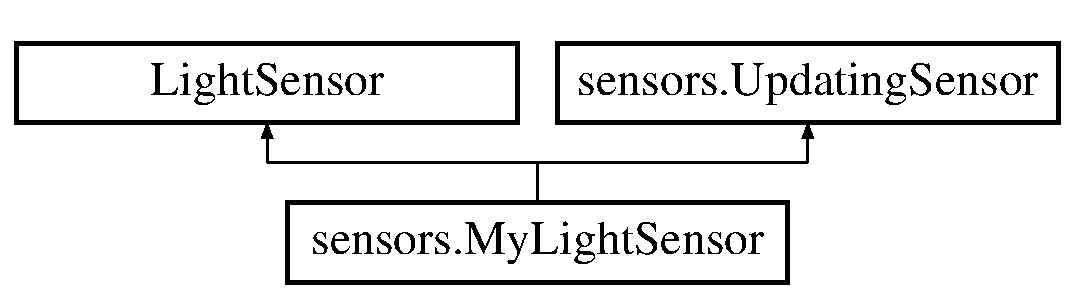
\includegraphics[height=2.000000cm]{classsensors_1_1_my_light_sensor}
\end{center}
\end{figure}
\subsection*{Public Member Functions}
\begin{DoxyCompactItemize}
\item 
\hyperlink{classsensors_1_1_my_light_sensor_a66871b7c407c55db943fa287f5a05546}{My\-Light\-Sensor} (Sensor\-Port sensorport, \hyperlink{enumsensors_1_1_position}{Position} position)
\item 
void \hyperlink{classsensors_1_1_my_light_sensor_a53d99d3eb2357a4a8bcaa4374a0cd322}{update\-State} ()
\item 
void \hyperlink{classsensors_1_1_my_light_sensor_a9f1363af86ed6a3684c0c5350893eaad}{add\-Listener} (\hyperlink{interfacesensors_1_1_light_sensor_listener}{Light\-Sensor\-Listener} listener)
\item 
void \hyperlink{classsensors_1_1_my_light_sensor_a5b7da6d342b87ca4dda0c22c29d352be}{delete\-Listener} (\hyperlink{interfacesensors_1_1_light_sensor_listener}{Light\-Sensor\-Listener} listener)
\item 
\hyperlink{enumsensors_1_1_sensor_type}{Sensor\-Type} \hyperlink{classsensors_1_1_my_light_sensor_a5a65a835bf1f749adf47e2f57d55047b}{get\-Sensor\-Type} ()
\end{DoxyCompactItemize}


\subsection{Detailed Description}
This class holds all the utilities to control the light sensor. Also this is a boundary class for the actual light sensor

\begin{DoxyAuthor}{Author}
Robert Bezem \href{mailto:robert.bezem@student.hu.nl}{\tt robert.\-bezem@student.\-hu.\-nl} 
\end{DoxyAuthor}
\begin{DoxyVersion}{Version}
1.\-0 
\end{DoxyVersion}
\begin{DoxySince}{Since}
01-\/04-\/2014 
\end{DoxySince}


\subsection{Constructor \& Destructor Documentation}
\hypertarget{classsensors_1_1_my_light_sensor_a66871b7c407c55db943fa287f5a05546}{\index{sensors\-::\-My\-Light\-Sensor@{sensors\-::\-My\-Light\-Sensor}!My\-Light\-Sensor@{My\-Light\-Sensor}}
\index{My\-Light\-Sensor@{My\-Light\-Sensor}!sensors::MyLightSensor@{sensors\-::\-My\-Light\-Sensor}}
\subsubsection[{My\-Light\-Sensor}]{\setlength{\rightskip}{0pt plus 5cm}sensors.\-My\-Light\-Sensor.\-My\-Light\-Sensor (
\begin{DoxyParamCaption}
\item[{Sensor\-Port}]{sensorport, }
\item[{{\bf Position}}]{position}
\end{DoxyParamCaption}
)}}\label{classsensors_1_1_my_light_sensor_a66871b7c407c55db943fa287f5a05546}
the constructor for the light sensor


\begin{DoxyParams}{Parameters}
{\em sensorport} & the port the light sensor is attached to on the N\-X\-T \\
\hline
{\em position} & the position the N\-X\-T \\
\hline
\end{DoxyParams}


\subsection{Member Function Documentation}
\hypertarget{classsensors_1_1_my_light_sensor_a9f1363af86ed6a3684c0c5350893eaad}{\index{sensors\-::\-My\-Light\-Sensor@{sensors\-::\-My\-Light\-Sensor}!add\-Listener@{add\-Listener}}
\index{add\-Listener@{add\-Listener}!sensors::MyLightSensor@{sensors\-::\-My\-Light\-Sensor}}
\subsubsection[{add\-Listener}]{\setlength{\rightskip}{0pt plus 5cm}void sensors.\-My\-Light\-Sensor.\-add\-Listener (
\begin{DoxyParamCaption}
\item[{{\bf Light\-Sensor\-Listener}}]{listener}
\end{DoxyParamCaption}
)}}\label{classsensors_1_1_my_light_sensor_a9f1363af86ed6a3684c0c5350893eaad}
adds the listener to the list of listeners


\begin{DoxyParams}{Parameters}
{\em listener} & the listener that is added \\
\hline
\end{DoxyParams}
\hypertarget{classsensors_1_1_my_light_sensor_a5b7da6d342b87ca4dda0c22c29d352be}{\index{sensors\-::\-My\-Light\-Sensor@{sensors\-::\-My\-Light\-Sensor}!delete\-Listener@{delete\-Listener}}
\index{delete\-Listener@{delete\-Listener}!sensors::MyLightSensor@{sensors\-::\-My\-Light\-Sensor}}
\subsubsection[{delete\-Listener}]{\setlength{\rightskip}{0pt plus 5cm}void sensors.\-My\-Light\-Sensor.\-delete\-Listener (
\begin{DoxyParamCaption}
\item[{{\bf Light\-Sensor\-Listener}}]{listener}
\end{DoxyParamCaption}
)}}\label{classsensors_1_1_my_light_sensor_a5b7da6d342b87ca4dda0c22c29d352be}
deletes the listener from the list of listeners


\begin{DoxyParams}{Parameters}
{\em listener} & the listener that has to be deleted \\
\hline
\end{DoxyParams}
\hypertarget{classsensors_1_1_my_light_sensor_a5a65a835bf1f749adf47e2f57d55047b}{\index{sensors\-::\-My\-Light\-Sensor@{sensors\-::\-My\-Light\-Sensor}!get\-Sensor\-Type@{get\-Sensor\-Type}}
\index{get\-Sensor\-Type@{get\-Sensor\-Type}!sensors::MyLightSensor@{sensors\-::\-My\-Light\-Sensor}}
\subsubsection[{get\-Sensor\-Type}]{\setlength{\rightskip}{0pt plus 5cm}{\bf Sensor\-Type} sensors.\-My\-Light\-Sensor.\-get\-Sensor\-Type (
\begin{DoxyParamCaption}
{}
\end{DoxyParamCaption}
)}}\label{classsensors_1_1_my_light_sensor_a5a65a835bf1f749adf47e2f57d55047b}
returns the type of sensor

\begin{DoxyReturn}{Returns}
S\-E\-N\-S\-O\-R\-T\-Y\-P\-E returns the type of the sensor 
\end{DoxyReturn}


Implements \hyperlink{interfacesensors_1_1_updating_sensor_aecdbf523b2bfe67a125b5587f71c4cf1}{sensors.\-Updating\-Sensor}.

\hypertarget{classsensors_1_1_my_light_sensor_a53d99d3eb2357a4a8bcaa4374a0cd322}{\index{sensors\-::\-My\-Light\-Sensor@{sensors\-::\-My\-Light\-Sensor}!update\-State@{update\-State}}
\index{update\-State@{update\-State}!sensors::MyLightSensor@{sensors\-::\-My\-Light\-Sensor}}
\subsubsection[{update\-State}]{\setlength{\rightskip}{0pt plus 5cm}void sensors.\-My\-Light\-Sensor.\-update\-State (
\begin{DoxyParamCaption}
{}
\end{DoxyParamCaption}
)}}\label{classsensors_1_1_my_light_sensor_a53d99d3eb2357a4a8bcaa4374a0cd322}
used to update the sensors value and if the have changed pass them to the listeners 

Implements \hyperlink{interfacesensors_1_1_updating_sensor_ac0b2a4f75f4a0e0f121a1aa6150d93a6}{sensors.\-Updating\-Sensor}.



The documentation for this class was generated from the following file\-:\begin{DoxyCompactItemize}
\item 
C\-:/\-Users/hp/git/the\-End/\-Eind\-Project/src/sensors/\hyperlink{_my_light_sensor_8java}{My\-Light\-Sensor.\-java}\end{DoxyCompactItemize}

\hypertarget{classsensors_1_1_my_ultra_sonic_sensor}{\section{sensors.\-My\-Ultra\-Sonic\-Sensor Class Reference}
\label{classsensors_1_1_my_ultra_sonic_sensor}\index{sensors.\-My\-Ultra\-Sonic\-Sensor@{sensors.\-My\-Ultra\-Sonic\-Sensor}}
}
Inheritance diagram for sensors.\-My\-Ultra\-Sonic\-Sensor\-:\begin{figure}[H]
\begin{center}
\leavevmode
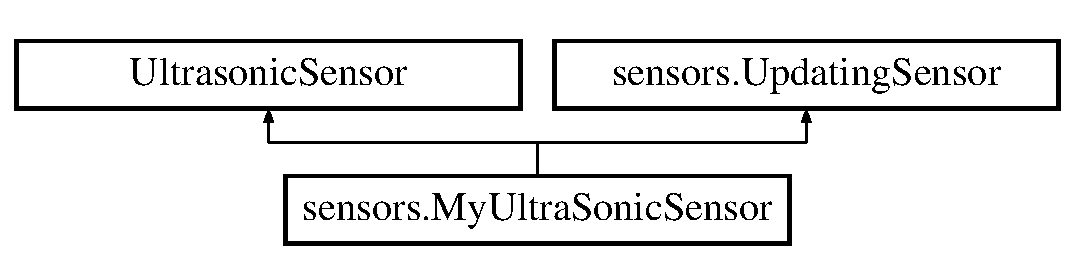
\includegraphics[height=2.000000cm]{classsensors_1_1_my_ultra_sonic_sensor}
\end{center}
\end{figure}
\subsection*{Public Member Functions}
\begin{DoxyCompactItemize}
\item 
\hyperlink{classsensors_1_1_my_ultra_sonic_sensor_a551fbaac3e8046b980afb5fcaad5ac7b}{My\-Ultra\-Sonic\-Sensor} (Sensor\-Port sensorport)
\item 
void \hyperlink{classsensors_1_1_my_ultra_sonic_sensor_a3c921c279968baa6629f9590cb5c5adc}{update\-State} ()
\item 
void \hyperlink{classsensors_1_1_my_ultra_sonic_sensor_a18264d10df33655322d6baa1e962052e}{add\-Listener} (\hyperlink{interfacesensors_1_1_ultrasonic_sensor_listener}{Ultrasonic\-Sensor\-Listener} ultrasonic\-Listener)
\item 
void \hyperlink{classsensors_1_1_my_ultra_sonic_sensor_aca8a150f651de6c00e88c6a7a0560431}{remove\-Listener} (\hyperlink{interfacesensors_1_1_ultrasonic_sensor_listener}{Ultrasonic\-Sensor\-Listener} ultrasonic\-Listener)
\item 
\hyperlink{enumsensors_1_1_sensor_type}{Sensor\-Type} \hyperlink{classsensors_1_1_my_ultra_sonic_sensor_a8ca6bc8d9caaa7bc63256bf37653bff8}{get\-Sensor\-Type} ()
\end{DoxyCompactItemize}


\subsection{Detailed Description}
This class holds all the utilities to control the ultrasonic sensor. Also this is a boundary class for the actual ultrasonic sensor

\begin{DoxyAuthor}{Author}
Robert Bezem \href{mailto:robert.bezem@student.hu.nl}{\tt robert.\-bezem@student.\-hu.\-nl} 
\end{DoxyAuthor}
\begin{DoxyVersion}{Version}
1.\-0 
\end{DoxyVersion}
\begin{DoxySince}{Since}
01-\/04-\/2014 
\end{DoxySince}


\subsection{Constructor \& Destructor Documentation}
\hypertarget{classsensors_1_1_my_ultra_sonic_sensor_a551fbaac3e8046b980afb5fcaad5ac7b}{\index{sensors\-::\-My\-Ultra\-Sonic\-Sensor@{sensors\-::\-My\-Ultra\-Sonic\-Sensor}!My\-Ultra\-Sonic\-Sensor@{My\-Ultra\-Sonic\-Sensor}}
\index{My\-Ultra\-Sonic\-Sensor@{My\-Ultra\-Sonic\-Sensor}!sensors::MyUltraSonicSensor@{sensors\-::\-My\-Ultra\-Sonic\-Sensor}}
\subsubsection[{My\-Ultra\-Sonic\-Sensor}]{\setlength{\rightskip}{0pt plus 5cm}sensors.\-My\-Ultra\-Sonic\-Sensor.\-My\-Ultra\-Sonic\-Sensor (
\begin{DoxyParamCaption}
\item[{Sensor\-Port}]{sensorport}
\end{DoxyParamCaption}
)}}\label{classsensors_1_1_my_ultra_sonic_sensor_a551fbaac3e8046b980afb5fcaad5ac7b}
Constructor for \hyperlink{interfacesensors_1_1_ultrasonic_sensor_listener}{Ultrasonic\-Sensor\-Listener}


\begin{DoxyParams}{Parameters}
{\em sensorport} & the given sensor port \\
\hline
\end{DoxyParams}


\subsection{Member Function Documentation}
\hypertarget{classsensors_1_1_my_ultra_sonic_sensor_a18264d10df33655322d6baa1e962052e}{\index{sensors\-::\-My\-Ultra\-Sonic\-Sensor@{sensors\-::\-My\-Ultra\-Sonic\-Sensor}!add\-Listener@{add\-Listener}}
\index{add\-Listener@{add\-Listener}!sensors::MyUltraSonicSensor@{sensors\-::\-My\-Ultra\-Sonic\-Sensor}}
\subsubsection[{add\-Listener}]{\setlength{\rightskip}{0pt plus 5cm}void sensors.\-My\-Ultra\-Sonic\-Sensor.\-add\-Listener (
\begin{DoxyParamCaption}
\item[{{\bf Ultrasonic\-Sensor\-Listener}}]{ultrasonic\-Listener}
\end{DoxyParamCaption}
)}}\label{classsensors_1_1_my_ultra_sonic_sensor_a18264d10df33655322d6baa1e962052e}
adds the \hyperlink{interfacesensors_1_1_ultrasonic_sensor_listener}{Ultrasonic\-Sensor\-Listener} to the listeners array


\begin{DoxyParams}{Parameters}
{\em ultrasonic\-Listener} & the given \hyperlink{interfacesensors_1_1_ultrasonic_sensor_listener}{Ultrasonic\-Sensor\-Listener} \\
\hline
\end{DoxyParams}
\hypertarget{classsensors_1_1_my_ultra_sonic_sensor_a8ca6bc8d9caaa7bc63256bf37653bff8}{\index{sensors\-::\-My\-Ultra\-Sonic\-Sensor@{sensors\-::\-My\-Ultra\-Sonic\-Sensor}!get\-Sensor\-Type@{get\-Sensor\-Type}}
\index{get\-Sensor\-Type@{get\-Sensor\-Type}!sensors::MyUltraSonicSensor@{sensors\-::\-My\-Ultra\-Sonic\-Sensor}}
\subsubsection[{get\-Sensor\-Type}]{\setlength{\rightskip}{0pt plus 5cm}{\bf Sensor\-Type} sensors.\-My\-Ultra\-Sonic\-Sensor.\-get\-Sensor\-Type (
\begin{DoxyParamCaption}
{}
\end{DoxyParamCaption}
)}}\label{classsensors_1_1_my_ultra_sonic_sensor_a8ca6bc8d9caaa7bc63256bf37653bff8}
returns the type of sensor

\begin{DoxyReturn}{Returns}
S\-E\-N\-S\-O\-R\-T\-Y\-P\-E returns the type of the sensor 
\end{DoxyReturn}


Implements \hyperlink{interfacesensors_1_1_updating_sensor_aecdbf523b2bfe67a125b5587f71c4cf1}{sensors.\-Updating\-Sensor}.

\hypertarget{classsensors_1_1_my_ultra_sonic_sensor_aca8a150f651de6c00e88c6a7a0560431}{\index{sensors\-::\-My\-Ultra\-Sonic\-Sensor@{sensors\-::\-My\-Ultra\-Sonic\-Sensor}!remove\-Listener@{remove\-Listener}}
\index{remove\-Listener@{remove\-Listener}!sensors::MyUltraSonicSensor@{sensors\-::\-My\-Ultra\-Sonic\-Sensor}}
\subsubsection[{remove\-Listener}]{\setlength{\rightskip}{0pt plus 5cm}void sensors.\-My\-Ultra\-Sonic\-Sensor.\-remove\-Listener (
\begin{DoxyParamCaption}
\item[{{\bf Ultrasonic\-Sensor\-Listener}}]{ultrasonic\-Listener}
\end{DoxyParamCaption}
)}}\label{classsensors_1_1_my_ultra_sonic_sensor_aca8a150f651de6c00e88c6a7a0560431}
removes the \hyperlink{interfacesensors_1_1_ultrasonic_sensor_listener}{Ultrasonic\-Sensor\-Listener} to the listeners array


\begin{DoxyParams}{Parameters}
{\em ultrasonic\-Listener} & the given \hyperlink{interfacesensors_1_1_ultrasonic_sensor_listener}{Ultrasonic\-Sensor\-Listener} \\
\hline
\end{DoxyParams}
\hypertarget{classsensors_1_1_my_ultra_sonic_sensor_a3c921c279968baa6629f9590cb5c5adc}{\index{sensors\-::\-My\-Ultra\-Sonic\-Sensor@{sensors\-::\-My\-Ultra\-Sonic\-Sensor}!update\-State@{update\-State}}
\index{update\-State@{update\-State}!sensors::MyUltraSonicSensor@{sensors\-::\-My\-Ultra\-Sonic\-Sensor}}
\subsubsection[{update\-State}]{\setlength{\rightskip}{0pt plus 5cm}void sensors.\-My\-Ultra\-Sonic\-Sensor.\-update\-State (
\begin{DoxyParamCaption}
{}
\end{DoxyParamCaption}
)}}\label{classsensors_1_1_my_ultra_sonic_sensor_a3c921c279968baa6629f9590cb5c5adc}
\begin{DoxySeeAlso}{See Also}
\hyperlink{interfacesensors_1_1_updating_sensor_ac0b2a4f75f4a0e0f121a1aa6150d93a6}{sensors.\-Updating\-Sensor\-::update\-State()} 
\end{DoxySeeAlso}


Implements \hyperlink{interfacesensors_1_1_updating_sensor_ac0b2a4f75f4a0e0f121a1aa6150d93a6}{sensors.\-Updating\-Sensor}.



The documentation for this class was generated from the following file\-:\begin{DoxyCompactItemize}
\item 
C\-:/\-Users/hp/git/the\-End/\-Eind\-Project/src/sensors/\hyperlink{_my_ultra_sonic_sensor_8java}{My\-Ultra\-Sonic\-Sensor.\-java}\end{DoxyCompactItemize}

\hypertarget{classcontrollers_1_1_obstruction_controller}{\section{controllers.\-Obstruction\-Controller Class Reference}
\label{classcontrollers_1_1_obstruction_controller}\index{controllers.\-Obstruction\-Controller@{controllers.\-Obstruction\-Controller}}
}
Inheritance diagram for controllers.\-Obstruction\-Controller\-:\begin{figure}[H]
\begin{center}
\leavevmode
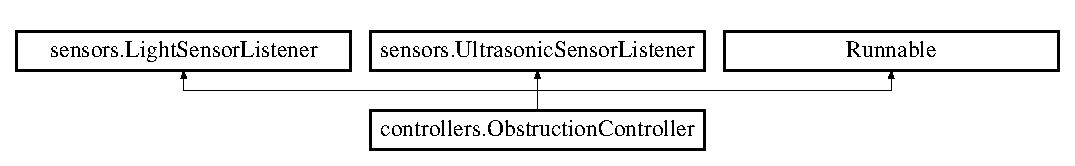
\includegraphics[height=1.786284cm]{classcontrollers_1_1_obstruction_controller}
\end{center}
\end{figure}
\subsection*{Public Member Functions}
\begin{DoxyCompactItemize}
\item 
\hyperlink{classcontrollers_1_1_obstruction_controller_a68a1a050f3f7a25a6b11565a1a19386d}{Obstruction\-Controller} (\hyperlink{classsensors_1_1_my_color_sensor}{My\-Color\-Sensor} cs, \hyperlink{classsensors_1_1_my_light_sensor}{My\-Light\-Sensor} ls, \hyperlink{classsensors_1_1_my_ultra_sonic_sensor}{My\-Ultra\-Sonic\-Sensor} us, \hyperlink{classgui_1_1_g_u_i}{G\-U\-I} gui)
\item 
void \hyperlink{classcontrollers_1_1_obstruction_controller_ab6f90766f733da01b7022b32f55b9d50}{run} ()
\item 
void \hyperlink{classcontrollers_1_1_obstruction_controller_a3b97c6803b754642db14268a7f0ce170}{ultra\-Sonic\-Changed} (\hyperlink{interfacesensors_1_1_updating_sensor}{Updating\-Sensor} us, float old\-Value, float new\-Value)
\item 
void \hyperlink{classcontrollers_1_1_obstruction_controller_ae8627b8e53bd16dcefeb5b84dfc55ee5}{light\-Sensor\-Changed} (\hyperlink{enumsensors_1_1_position}{Position} position, \hyperlink{interfacesensors_1_1_updating_sensor}{Updating\-Sensor} updatingsensor, float old\-Value, float new\-Value)
\end{DoxyCompactItemize}


\subsection{Detailed Description}
This class will evade objects

\begin{DoxyAuthor}{Author}
Robert Bezem \href{mailto:robert.bezem@student.hu.nl}{\tt robert.\-bezem@student.\-hu.\-nl} 
\end{DoxyAuthor}
\begin{DoxyVersion}{Version}
1.\-2 
\end{DoxyVersion}
\begin{DoxySince}{Since}
01-\/04-\/2014 
\end{DoxySince}


\subsection{Constructor \& Destructor Documentation}
\hypertarget{classcontrollers_1_1_obstruction_controller_a68a1a050f3f7a25a6b11565a1a19386d}{\index{controllers\-::\-Obstruction\-Controller@{controllers\-::\-Obstruction\-Controller}!Obstruction\-Controller@{Obstruction\-Controller}}
\index{Obstruction\-Controller@{Obstruction\-Controller}!controllers::ObstructionController@{controllers\-::\-Obstruction\-Controller}}
\subsubsection[{Obstruction\-Controller}]{\setlength{\rightskip}{0pt plus 5cm}controllers.\-Obstruction\-Controller.\-Obstruction\-Controller (
\begin{DoxyParamCaption}
\item[{{\bf My\-Color\-Sensor}}]{cs, }
\item[{{\bf My\-Light\-Sensor}}]{ls, }
\item[{{\bf My\-Ultra\-Sonic\-Sensor}}]{us, }
\item[{{\bf G\-U\-I}}]{gui}
\end{DoxyParamCaption}
)}}\label{classcontrollers_1_1_obstruction_controller_a68a1a050f3f7a25a6b11565a1a19386d}
The constructor for the \hyperlink{classcontrollers_1_1_obstruction_controller}{Obstruction\-Controller} class


\begin{DoxyParams}{Parameters}
{\em cs} & The color sensor on the robot \\
\hline
{\em ls} & The light sensor on the robot \\
\hline
{\em us} & The ultrasonic sensor on the robot \\
\hline
{\em gui} & The G\-U\-I that is used \\
\hline
\end{DoxyParams}


\subsection{Member Function Documentation}
\hypertarget{classcontrollers_1_1_obstruction_controller_ae8627b8e53bd16dcefeb5b84dfc55ee5}{\index{controllers\-::\-Obstruction\-Controller@{controllers\-::\-Obstruction\-Controller}!light\-Sensor\-Changed@{light\-Sensor\-Changed}}
\index{light\-Sensor\-Changed@{light\-Sensor\-Changed}!controllers::ObstructionController@{controllers\-::\-Obstruction\-Controller}}
\subsubsection[{light\-Sensor\-Changed}]{\setlength{\rightskip}{0pt plus 5cm}void controllers.\-Obstruction\-Controller.\-light\-Sensor\-Changed (
\begin{DoxyParamCaption}
\item[{{\bf Position}}]{position, }
\item[{{\bf Updating\-Sensor}}]{updatingsensor, }
\item[{float}]{old\-Value, }
\item[{float}]{new\-Value}
\end{DoxyParamCaption}
)}}\label{classcontrollers_1_1_obstruction_controller_ae8627b8e53bd16dcefeb5b84dfc55ee5}
If the measured value from the light sensor changes this method is called. When called this method checks the position of the sensor who called this method, and sets the attribute corresponding to the position.

\begin{DoxySeeAlso}{See Also}
\hyperlink{interfacesensors_1_1_light_sensor_listener_ad454a7e5082bc820b4cc27cf173a111a}{sensors.\-Light\-Sensor\-Listener\-::light\-Sensor\-Changed}(sensors.\-Sensor\-Position, \hyperlink{interfacesensors_1_1_updating_sensor}{sensors.\-Updating\-Sensor}, float, float) 
\end{DoxySeeAlso}


Implements \hyperlink{interfacesensors_1_1_light_sensor_listener_ad454a7e5082bc820b4cc27cf173a111a}{sensors.\-Light\-Sensor\-Listener}.

\hypertarget{classcontrollers_1_1_obstruction_controller_ab6f90766f733da01b7022b32f55b9d50}{\index{controllers\-::\-Obstruction\-Controller@{controllers\-::\-Obstruction\-Controller}!run@{run}}
\index{run@{run}!controllers::ObstructionController@{controllers\-::\-Obstruction\-Controller}}
\subsubsection[{run}]{\setlength{\rightskip}{0pt plus 5cm}void controllers.\-Obstruction\-Controller.\-run (
\begin{DoxyParamCaption}
{}
\end{DoxyParamCaption}
)}}\label{classcontrollers_1_1_obstruction_controller_ab6f90766f733da01b7022b32f55b9d50}
\hypertarget{classcontrollers_1_1_obstruction_controller_a3b97c6803b754642db14268a7f0ce170}{\index{controllers\-::\-Obstruction\-Controller@{controllers\-::\-Obstruction\-Controller}!ultra\-Sonic\-Changed@{ultra\-Sonic\-Changed}}
\index{ultra\-Sonic\-Changed@{ultra\-Sonic\-Changed}!controllers::ObstructionController@{controllers\-::\-Obstruction\-Controller}}
\subsubsection[{ultra\-Sonic\-Changed}]{\setlength{\rightskip}{0pt plus 5cm}void controllers.\-Obstruction\-Controller.\-ultra\-Sonic\-Changed (
\begin{DoxyParamCaption}
\item[{{\bf Updating\-Sensor}}]{us, }
\item[{float}]{old\-Value, }
\item[{float}]{new\-Value}
\end{DoxyParamCaption}
)}}\label{classcontrollers_1_1_obstruction_controller_a3b97c6803b754642db14268a7f0ce170}
If the measured value from the ultrasonic sensor changes this method is called. When called this method checks of the new value is smaller than the safe value, if that's true the robot displays a message and starts a evasive maneuver. When the new value is bigger than the save distance any messages on the display disappear. $\ast$

\begin{DoxySeeAlso}{See Also}
\hyperlink{interfacesensors_1_1_ultrasonic_sensor_listener_ac66510bffddde1ed90f98b5fe1858f21}{sensors.\-Ultrasonic\-Sensor\-Listener\-::ultra\-Sonic\-Changed}(\hyperlink{interfacesensors_1_1_updating_sensor}{sensors.\-Updating\-Sensor}, float, float) 
\end{DoxySeeAlso}


Implements \hyperlink{interfacesensors_1_1_ultrasonic_sensor_listener_ac66510bffddde1ed90f98b5fe1858f21}{sensors.\-Ultrasonic\-Sensor\-Listener}.



The documentation for this class was generated from the following file\-:\begin{DoxyCompactItemize}
\item 
C\-:/\-Users/hp/git/the\-End/\-Eind\-Project/src/controllers/\hyperlink{_obstruction_controller_8java}{Obstruction\-Controller.\-java}\end{DoxyCompactItemize}

\hypertarget{enumsensors_1_1_position}{\section{sensors.\-Position Enum Reference}
\label{enumsensors_1_1_position}\index{sensors.\-Position@{sensors.\-Position}}
}
\subsection*{Public Attributes}
\begin{DoxyCompactItemize}
\item 
\hyperlink{enumsensors_1_1_position_a6f0d6987f9fb0f870c585227a2e40c27}{Left}
\end{DoxyCompactItemize}


\subsection{Detailed Description}
These enum's are used to explain the location of a certain sensor on the frame of the robot

\begin{DoxyAuthor}{Author}
Jacob Visser \href{mailto:Jacob.Visser@student.hu.nl}{\tt Jacob.\-Visser@student.\-hu.\-nl} 

Robert Bezem \href{mailto:robert.bezem@student.hu.nl}{\tt robert.\-bezem@student.\-hu.\-nl} 
\end{DoxyAuthor}
\begin{DoxyVersion}{Version}
1.\-0 
\end{DoxyVersion}
\begin{DoxySince}{Since}
01-\/04-\/2014 
\end{DoxySince}


\subsection{Member Data Documentation}
\hypertarget{enumsensors_1_1_position_a6f0d6987f9fb0f870c585227a2e40c27}{\index{sensors\-::\-Position@{sensors\-::\-Position}!Left@{Left}}
\index{Left@{Left}!sensors::Position@{sensors\-::\-Position}}
\subsubsection[{Left}]{\setlength{\rightskip}{0pt plus 5cm}sensors.\-Position.\-Left}}\label{enumsensors_1_1_position_a6f0d6987f9fb0f870c585227a2e40c27}


The documentation for this enum was generated from the following file\-:\begin{DoxyCompactItemize}
\item 
C\-:/\-Users/hp/git/the\-End/\-Eind\-Project/src/sensors/\hyperlink{_position_8java}{Position.\-java}\end{DoxyCompactItemize}

\hypertarget{classsensors_1_1_sensor_handler}{\section{sensors.\-Sensor\-Handler Class Reference}
\label{classsensors_1_1_sensor_handler}\index{sensors.\-Sensor\-Handler@{sensors.\-Sensor\-Handler}}
}
Inheritance diagram for sensors.\-Sensor\-Handler\-:\begin{figure}[H]
\begin{center}
\leavevmode
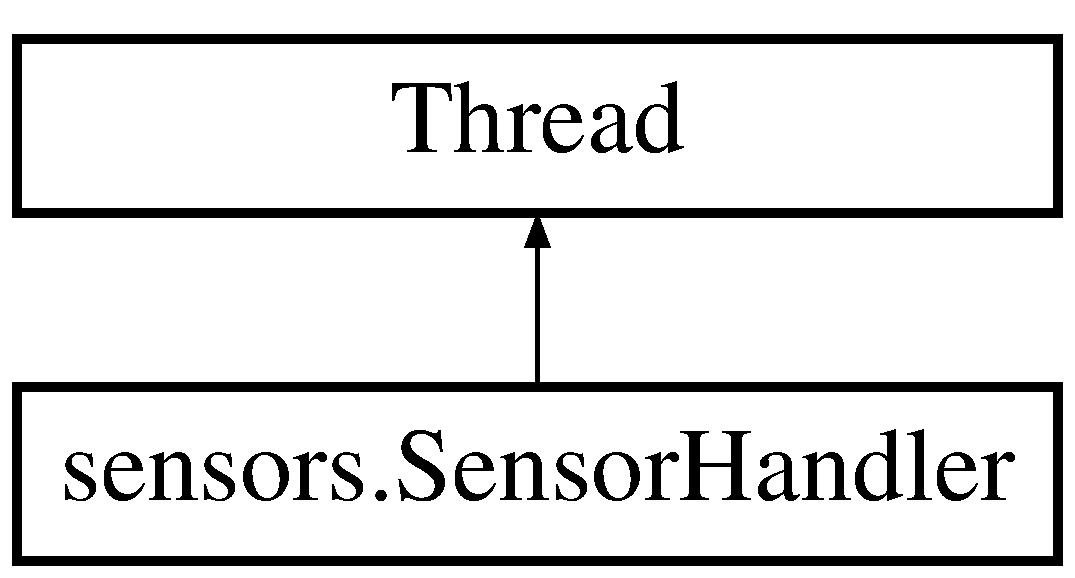
\includegraphics[height=2.000000cm]{classsensors_1_1_sensor_handler}
\end{center}
\end{figure}
\subsection*{Public Member Functions}
\begin{DoxyCompactItemize}
\item 
void \hyperlink{classsensors_1_1_sensor_handler_abf934699cf3b07eec525bd47acc887e7}{run} ()
\item 
void \hyperlink{classsensors_1_1_sensor_handler_a7ab54a96695c7e0374cebfca2dd6cc4d}{add\-Sensor} (\hyperlink{interfacesensors_1_1_updating_sensor}{Updating\-Sensor} updating\-Sensor)
\item 
void \hyperlink{classsensors_1_1_sensor_handler_a03c2a4215b0767097561dc76df0cb803}{remove\-Sensor} (\hyperlink{interfacesensors_1_1_updating_sensor}{Updating\-Sensor} updating\-Sensor)
\end{DoxyCompactItemize}
\subsection*{Static Public Member Functions}
\begin{DoxyCompactItemize}
\item 
static \hyperlink{classsensors_1_1_sensor_handler}{Sensor\-Handler} \hyperlink{classsensors_1_1_sensor_handler_ad3f54cd330faf0f9e999201b7fb347f0}{get\-Instance} ()
\end{DoxyCompactItemize}


\subsection{Detailed Description}
This class handles all the sensors and requests updates of each sensor every set period of time

\begin{DoxyAuthor}{Author}
Robert Bezem \href{mailto:robert.bezem@student.hu.nl}{\tt robert.\-bezem@student.\-hu.\-nl} 
\end{DoxyAuthor}
\begin{DoxyVersion}{Version}
1.\-0 
\end{DoxyVersion}
\begin{DoxySince}{Since}
01-\/04-\/2014 
\end{DoxySince}


\subsection{Member Function Documentation}
\hypertarget{classsensors_1_1_sensor_handler_a7ab54a96695c7e0374cebfca2dd6cc4d}{\index{sensors\-::\-Sensor\-Handler@{sensors\-::\-Sensor\-Handler}!add\-Sensor@{add\-Sensor}}
\index{add\-Sensor@{add\-Sensor}!sensors::SensorHandler@{sensors\-::\-Sensor\-Handler}}
\subsubsection[{add\-Sensor}]{\setlength{\rightskip}{0pt plus 5cm}void sensors.\-Sensor\-Handler.\-add\-Sensor (
\begin{DoxyParamCaption}
\item[{{\bf Updating\-Sensor}}]{updating\-Sensor}
\end{DoxyParamCaption}
)}}\label{classsensors_1_1_sensor_handler_a7ab54a96695c7e0374cebfca2dd6cc4d}
adds 'updating\-Sensor' to the list of sensors registered to this handler


\begin{DoxyParams}{Parameters}
{\em updating\-Sensor} & the sensor that has to be added \\
\hline
\end{DoxyParams}
\hypertarget{classsensors_1_1_sensor_handler_ad3f54cd330faf0f9e999201b7fb347f0}{\index{sensors\-::\-Sensor\-Handler@{sensors\-::\-Sensor\-Handler}!get\-Instance@{get\-Instance}}
\index{get\-Instance@{get\-Instance}!sensors::SensorHandler@{sensors\-::\-Sensor\-Handler}}
\subsubsection[{get\-Instance}]{\setlength{\rightskip}{0pt plus 5cm}static {\bf Sensor\-Handler} sensors.\-Sensor\-Handler.\-get\-Instance (
\begin{DoxyParamCaption}
{}
\end{DoxyParamCaption}
)\hspace{0.3cm}{\ttfamily [static]}}}\label{classsensors_1_1_sensor_handler_ad3f54cd330faf0f9e999201b7fb347f0}
gives instance to the \hyperlink{classsensors_1_1_sensor_handler}{Sensor\-Handler}

\begin{DoxyReturn}{Returns}
\hyperlink{classsensors_1_1_sensor_handler}{Sensor\-Handler} returns the instance of \hyperlink{classsensors_1_1_sensor_handler}{Sensor\-Handler} 
\end{DoxyReturn}
\hypertarget{classsensors_1_1_sensor_handler_a03c2a4215b0767097561dc76df0cb803}{\index{sensors\-::\-Sensor\-Handler@{sensors\-::\-Sensor\-Handler}!remove\-Sensor@{remove\-Sensor}}
\index{remove\-Sensor@{remove\-Sensor}!sensors::SensorHandler@{sensors\-::\-Sensor\-Handler}}
\subsubsection[{remove\-Sensor}]{\setlength{\rightskip}{0pt plus 5cm}void sensors.\-Sensor\-Handler.\-remove\-Sensor (
\begin{DoxyParamCaption}
\item[{{\bf Updating\-Sensor}}]{updating\-Sensor}
\end{DoxyParamCaption}
)}}\label{classsensors_1_1_sensor_handler_a03c2a4215b0767097561dc76df0cb803}
removes 'updating\-Sensor' to the list of sensors registered to this handler


\begin{DoxyParams}{Parameters}
{\em updating\-Sensor} & the sensor that has to be removed \\
\hline
\end{DoxyParams}
\hypertarget{classsensors_1_1_sensor_handler_abf934699cf3b07eec525bd47acc887e7}{\index{sensors\-::\-Sensor\-Handler@{sensors\-::\-Sensor\-Handler}!run@{run}}
\index{run@{run}!sensors::SensorHandler@{sensors\-::\-Sensor\-Handler}}
\subsubsection[{run}]{\setlength{\rightskip}{0pt plus 5cm}void sensors.\-Sensor\-Handler.\-run (
\begin{DoxyParamCaption}
{}
\end{DoxyParamCaption}
)}}\label{classsensors_1_1_sensor_handler_abf934699cf3b07eec525bd47acc887e7}
updates all the added sensors 

The documentation for this class was generated from the following file\-:\begin{DoxyCompactItemize}
\item 
C\-:/\-Users/hp/git/the\-End/\-Eind\-Project/src/sensors/\hyperlink{_sensor_handler_8java}{Sensor\-Handler.\-java}\end{DoxyCompactItemize}

\hypertarget{enumsensors_1_1_sensor_type}{\section{sensors.\-Sensor\-Type Enum Reference}
\label{enumsensors_1_1_sensor_type}\index{sensors.\-Sensor\-Type@{sensors.\-Sensor\-Type}}
}
\subsection*{Public Attributes}
\begin{DoxyCompactItemize}
\item 
\hyperlink{enumsensors_1_1_sensor_type_a56c9a2b279f1d909323b79f8ef272ff7}{Colorsensor}
\item 
\hyperlink{enumsensors_1_1_sensor_type_a6438e9ee7c60fcd103234e28e986c1ea}{Lightsensor}
\item 
\hyperlink{enumsensors_1_1_sensor_type_a850fa290a12e42dafa929ff12bdcf574}{Ultrasonicsensor}
\item 
\hyperlink{enumsensors_1_1_sensor_type_ad4009ea0d42269e90107270a4eaeb372}{Pressuresensor}
\end{DoxyCompactItemize}


\subsection{Detailed Description}
\begin{DoxyAuthor}{Author}
Robert Bezem \href{mailto:robert.bezem@student.hu.nl}{\tt robert.\-bezem@student.\-hu.\-nl} 
\end{DoxyAuthor}
\begin{DoxyVersion}{Version}
1.\-0 
\end{DoxyVersion}
\begin{DoxySince}{Since}
02-\/04-\/2014 
\end{DoxySince}


\subsection{Member Data Documentation}
\hypertarget{enumsensors_1_1_sensor_type_a56c9a2b279f1d909323b79f8ef272ff7}{\index{sensors\-::\-Sensor\-Type@{sensors\-::\-Sensor\-Type}!Colorsensor@{Colorsensor}}
\index{Colorsensor@{Colorsensor}!sensors::SensorType@{sensors\-::\-Sensor\-Type}}
\subsubsection[{Colorsensor}]{\setlength{\rightskip}{0pt plus 5cm}sensors.\-Sensor\-Type.\-Colorsensor}}\label{enumsensors_1_1_sensor_type_a56c9a2b279f1d909323b79f8ef272ff7}
\hypertarget{enumsensors_1_1_sensor_type_a6438e9ee7c60fcd103234e28e986c1ea}{\index{sensors\-::\-Sensor\-Type@{sensors\-::\-Sensor\-Type}!Lightsensor@{Lightsensor}}
\index{Lightsensor@{Lightsensor}!sensors::SensorType@{sensors\-::\-Sensor\-Type}}
\subsubsection[{Lightsensor}]{\setlength{\rightskip}{0pt plus 5cm}sensors.\-Sensor\-Type.\-Lightsensor}}\label{enumsensors_1_1_sensor_type_a6438e9ee7c60fcd103234e28e986c1ea}
\hypertarget{enumsensors_1_1_sensor_type_ad4009ea0d42269e90107270a4eaeb372}{\index{sensors\-::\-Sensor\-Type@{sensors\-::\-Sensor\-Type}!Pressuresensor@{Pressuresensor}}
\index{Pressuresensor@{Pressuresensor}!sensors::SensorType@{sensors\-::\-Sensor\-Type}}
\subsubsection[{Pressuresensor}]{\setlength{\rightskip}{0pt plus 5cm}sensors.\-Sensor\-Type.\-Pressuresensor}}\label{enumsensors_1_1_sensor_type_ad4009ea0d42269e90107270a4eaeb372}
\hypertarget{enumsensors_1_1_sensor_type_a850fa290a12e42dafa929ff12bdcf574}{\index{sensors\-::\-Sensor\-Type@{sensors\-::\-Sensor\-Type}!Ultrasonicsensor@{Ultrasonicsensor}}
\index{Ultrasonicsensor@{Ultrasonicsensor}!sensors::SensorType@{sensors\-::\-Sensor\-Type}}
\subsubsection[{Ultrasonicsensor}]{\setlength{\rightskip}{0pt plus 5cm}sensors.\-Sensor\-Type.\-Ultrasonicsensor}}\label{enumsensors_1_1_sensor_type_a850fa290a12e42dafa929ff12bdcf574}


The documentation for this enum was generated from the following file\-:\begin{DoxyCompactItemize}
\item 
C\-:/\-Users/hp/git/the\-End/\-Eind\-Project/src/sensors/\hyperlink{_sensor_type_8java}{Sensor\-Type.\-java}\end{DoxyCompactItemize}

\hypertarget{interfacesensors_1_1_ultrasonic_sensor_listener}{\section{sensors.\-Ultrasonic\-Sensor\-Listener Interface Reference}
\label{interfacesensors_1_1_ultrasonic_sensor_listener}\index{sensors.\-Ultrasonic\-Sensor\-Listener@{sensors.\-Ultrasonic\-Sensor\-Listener}}
}
Inheritance diagram for sensors.\-Ultrasonic\-Sensor\-Listener\-:\begin{figure}[H]
\begin{center}
\leavevmode
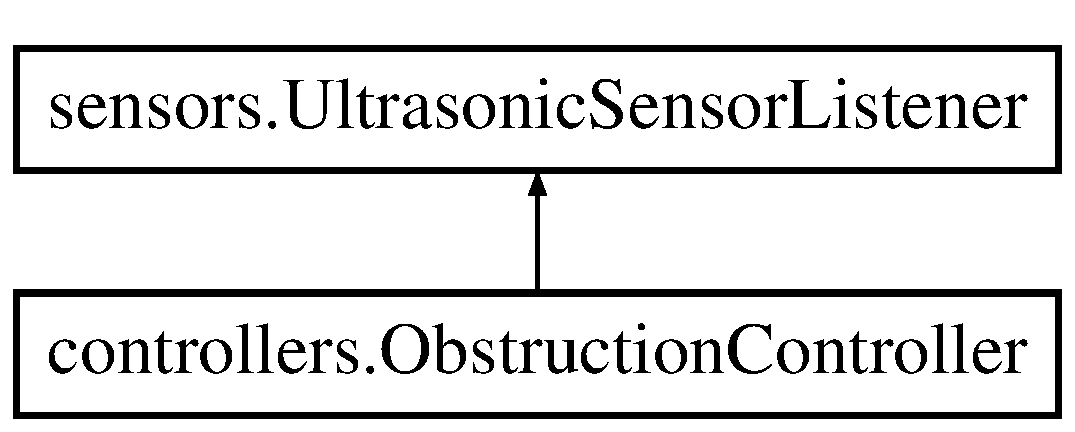
\includegraphics[height=2.000000cm]{interfacesensors_1_1_ultrasonic_sensor_listener}
\end{center}
\end{figure}
\subsection*{Public Member Functions}
\begin{DoxyCompactItemize}
\item 
void \hyperlink{interfacesensors_1_1_ultrasonic_sensor_listener_ac66510bffddde1ed90f98b5fe1858f21}{ultra\-Sonic\-Changed} (\hyperlink{interfacesensors_1_1_updating_sensor}{Updating\-Sensor} us, float old\-Value, float new\-Value)
\end{DoxyCompactItemize}


\subsection{Detailed Description}
This is the ultrasonic sensor listener interface

\begin{DoxyAuthor}{Author}
Robert Bezem \href{mailto:robert.bezem@student.hu.nl}{\tt robert.\-bezem@student.\-hu.\-nl} 
\end{DoxyAuthor}
\begin{DoxyVersion}{Version}
1.\-0 
\end{DoxyVersion}
\begin{DoxySince}{Since}
01-\/04-\/2014 
\end{DoxySince}


\subsection{Member Function Documentation}
\hypertarget{interfacesensors_1_1_ultrasonic_sensor_listener_ac66510bffddde1ed90f98b5fe1858f21}{\index{sensors\-::\-Ultrasonic\-Sensor\-Listener@{sensors\-::\-Ultrasonic\-Sensor\-Listener}!ultra\-Sonic\-Changed@{ultra\-Sonic\-Changed}}
\index{ultra\-Sonic\-Changed@{ultra\-Sonic\-Changed}!sensors::UltrasonicSensorListener@{sensors\-::\-Ultrasonic\-Sensor\-Listener}}
\subsubsection[{ultra\-Sonic\-Changed}]{\setlength{\rightskip}{0pt plus 5cm}void sensors.\-Ultrasonic\-Sensor\-Listener.\-ultra\-Sonic\-Changed (
\begin{DoxyParamCaption}
\item[{{\bf Updating\-Sensor}}]{us, }
\item[{float}]{old\-Value, }
\item[{float}]{new\-Value}
\end{DoxyParamCaption}
)}}\label{interfacesensors_1_1_ultrasonic_sensor_listener_ac66510bffddde1ed90f98b5fe1858f21}
When implemented this method can be called to do something when the measured value from the ultrasonic sensor changes


\begin{DoxyParams}{Parameters}
{\em us} & The sensor from which the value is changed \\
\hline
{\em old\-Value} & The old value from the sensor \\
\hline
{\em new\-Value} & The new value from the sensor \\
\hline
\end{DoxyParams}


Implemented in \hyperlink{classcontrollers_1_1_obstruction_controller_a3b97c6803b754642db14268a7f0ce170}{controllers.\-Obstruction\-Controller}.



The documentation for this interface was generated from the following file\-:\begin{DoxyCompactItemize}
\item 
C\-:/\-Users/hp/git/the\-End/\-Eind\-Project/src/sensors/\hyperlink{_ultrasonic_sensor_listener_8java}{Ultrasonic\-Sensor\-Listener.\-java}\end{DoxyCompactItemize}

\hypertarget{interfacesensors_1_1_updating_sensor}{\section{sensors.\-Updating\-Sensor Interface Reference}
\label{interfacesensors_1_1_updating_sensor}\index{sensors.\-Updating\-Sensor@{sensors.\-Updating\-Sensor}}
}
Inheritance diagram for sensors.\-Updating\-Sensor\-:\begin{figure}[H]
\begin{center}
\leavevmode
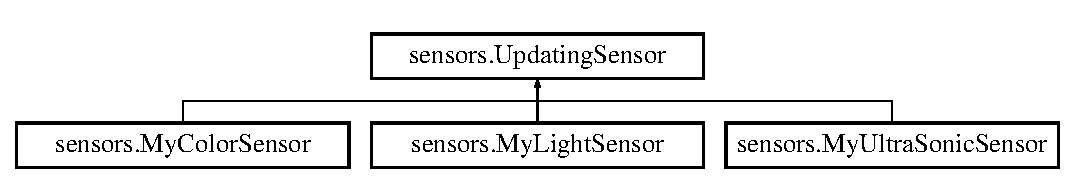
\includegraphics[height=2.000000cm]{interfacesensors_1_1_updating_sensor}
\end{center}
\end{figure}
\subsection*{Public Member Functions}
\begin{DoxyCompactItemize}
\item 
void \hyperlink{interfacesensors_1_1_updating_sensor_ac0b2a4f75f4a0e0f121a1aa6150d93a6}{update\-State} ()
\item 
\hyperlink{enumsensors_1_1_sensor_type}{Sensor\-Type} \hyperlink{interfacesensors_1_1_updating_sensor_aecdbf523b2bfe67a125b5587f71c4cf1}{get\-Sensor\-Type} ()
\end{DoxyCompactItemize}


\subsection{Detailed Description}
This is the updating\-Sensor interface which is implemented by all sensors so that the sensor\-Handler can update all sensors

\begin{DoxyAuthor}{Author}
Robert Bezem \href{mailto:robert.bezem@student.hu.nl}{\tt robert.\-bezem@student.\-hu.\-nl} 
\end{DoxyAuthor}
\begin{DoxyVersion}{Version}
1.\-0 
\end{DoxyVersion}
\begin{DoxySince}{Since}
01-\/04-\/2014 
\end{DoxySince}


\subsection{Member Function Documentation}
\hypertarget{interfacesensors_1_1_updating_sensor_aecdbf523b2bfe67a125b5587f71c4cf1}{\index{sensors\-::\-Updating\-Sensor@{sensors\-::\-Updating\-Sensor}!get\-Sensor\-Type@{get\-Sensor\-Type}}
\index{get\-Sensor\-Type@{get\-Sensor\-Type}!sensors::UpdatingSensor@{sensors\-::\-Updating\-Sensor}}
\subsubsection[{get\-Sensor\-Type}]{\setlength{\rightskip}{0pt plus 5cm}{\bf Sensor\-Type} sensors.\-Updating\-Sensor.\-get\-Sensor\-Type (
\begin{DoxyParamCaption}
{}
\end{DoxyParamCaption}
)}}\label{interfacesensors_1_1_updating_sensor_aecdbf523b2bfe67a125b5587f71c4cf1}
Every sensor is from a different type, with this method you can determine the sensor type 

Implemented in \hyperlink{classsensors_1_1_my_color_sensor_a62eaf9476cb88ab8e77f720e7953c6cd}{sensors.\-My\-Color\-Sensor}, \hyperlink{classsensors_1_1_my_light_sensor_a5a65a835bf1f749adf47e2f57d55047b}{sensors.\-My\-Light\-Sensor}, and \hyperlink{classsensors_1_1_my_ultra_sonic_sensor_a8ca6bc8d9caaa7bc63256bf37653bff8}{sensors.\-My\-Ultra\-Sonic\-Sensor}.

\hypertarget{interfacesensors_1_1_updating_sensor_ac0b2a4f75f4a0e0f121a1aa6150d93a6}{\index{sensors\-::\-Updating\-Sensor@{sensors\-::\-Updating\-Sensor}!update\-State@{update\-State}}
\index{update\-State@{update\-State}!sensors::UpdatingSensor@{sensors\-::\-Updating\-Sensor}}
\subsubsection[{update\-State}]{\setlength{\rightskip}{0pt plus 5cm}void sensors.\-Updating\-Sensor.\-update\-State (
\begin{DoxyParamCaption}
{}
\end{DoxyParamCaption}
)}}\label{interfacesensors_1_1_updating_sensor_ac0b2a4f75f4a0e0f121a1aa6150d93a6}
When implemented this method can update the measured values from a sensor 

Implemented in \hyperlink{classsensors_1_1_my_color_sensor_a17324aa0de8fa9ab45bb2c1450e0119a}{sensors.\-My\-Color\-Sensor}, \hyperlink{classsensors_1_1_my_light_sensor_a53d99d3eb2357a4a8bcaa4374a0cd322}{sensors.\-My\-Light\-Sensor}, and \hyperlink{classsensors_1_1_my_ultra_sonic_sensor_a3c921c279968baa6629f9590cb5c5adc}{sensors.\-My\-Ultra\-Sonic\-Sensor}.



The documentation for this interface was generated from the following file\-:\begin{DoxyCompactItemize}
\item 
C\-:/\-Users/hp/git/the\-End/\-Eind\-Project/src/sensors/\hyperlink{_updating_sensor_8java}{Updating\-Sensor.\-java}\end{DoxyCompactItemize}

\chapter{File Documentation}
\hypertarget{_calibration_controller_8java}{\section{C\-:/\-Users/hp/git/the\-End/\-Eind\-Project/src/controllers/\-Calibration\-Controller.java File Reference}
\label{_calibration_controller_8java}\index{C\-:/\-Users/hp/git/the\-End/\-Eind\-Project/src/controllers/\-Calibration\-Controller.\-java@{C\-:/\-Users/hp/git/the\-End/\-Eind\-Project/src/controllers/\-Calibration\-Controller.\-java}}
}
\subsection*{Classes}
\begin{DoxyCompactItemize}
\item 
class \hyperlink{classcontrollers_1_1_calibration_controller}{controllers.\-Calibration\-Controller}
\end{DoxyCompactItemize}
\subsection*{Packages}
\begin{DoxyCompactItemize}
\item 
package \hyperlink{namespacecontrollers}{controllers}
\end{DoxyCompactItemize}

\hypertarget{_line_follow_controller_8java}{\section{C\-:/\-Users/hp/git/the\-End/\-Eind\-Project/src/controllers/\-Line\-Follow\-Controller.java File Reference}
\label{_line_follow_controller_8java}\index{C\-:/\-Users/hp/git/the\-End/\-Eind\-Project/src/controllers/\-Line\-Follow\-Controller.\-java@{C\-:/\-Users/hp/git/the\-End/\-Eind\-Project/src/controllers/\-Line\-Follow\-Controller.\-java}}
}
\subsection*{Classes}
\begin{DoxyCompactItemize}
\item 
class \hyperlink{classcontrollers_1_1_line_follow_controller}{controllers.\-Line\-Follow\-Controller}
\end{DoxyCompactItemize}
\subsection*{Packages}
\begin{DoxyCompactItemize}
\item 
package \hyperlink{namespacecontrollers}{controllers}
\end{DoxyCompactItemize}

\hypertarget{_obstruction_controller_8java}{\section{C\-:/\-Users/hp/git/the\-End/\-Eind\-Project/src/controllers/\-Obstruction\-Controller.java File Reference}
\label{_obstruction_controller_8java}\index{C\-:/\-Users/hp/git/the\-End/\-Eind\-Project/src/controllers/\-Obstruction\-Controller.\-java@{C\-:/\-Users/hp/git/the\-End/\-Eind\-Project/src/controllers/\-Obstruction\-Controller.\-java}}
}
\subsection*{Classes}
\begin{DoxyCompactItemize}
\item 
class \hyperlink{classcontrollers_1_1_obstruction_controller}{controllers.\-Obstruction\-Controller}
\end{DoxyCompactItemize}
\subsection*{Packages}
\begin{DoxyCompactItemize}
\item 
package \hyperlink{namespacecontrollers}{controllers}
\end{DoxyCompactItemize}

\hypertarget{_g_u_i_8java}{\section{C\-:/\-Users/hp/git/the\-End/\-Eind\-Project/src/gui/\-G\-U\-I.java File Reference}
\label{_g_u_i_8java}\index{C\-:/\-Users/hp/git/the\-End/\-Eind\-Project/src/gui/\-G\-U\-I.\-java@{C\-:/\-Users/hp/git/the\-End/\-Eind\-Project/src/gui/\-G\-U\-I.\-java}}
}
\subsection*{Classes}
\begin{DoxyCompactItemize}
\item 
class \hyperlink{classgui_1_1_g_u_i}{gui.\-G\-U\-I}
\end{DoxyCompactItemize}
\subsection*{Packages}
\begin{DoxyCompactItemize}
\item 
package \hyperlink{namespacegui}{gui}
\end{DoxyCompactItemize}

\hypertarget{_icons_8java}{\section{C\-:/\-Users/hp/git/the\-End/\-Eind\-Project/src/gui/\-Icons.java File Reference}
\label{_icons_8java}\index{C\-:/\-Users/hp/git/the\-End/\-Eind\-Project/src/gui/\-Icons.\-java@{C\-:/\-Users/hp/git/the\-End/\-Eind\-Project/src/gui/\-Icons.\-java}}
}
\subsection*{Classes}
\begin{DoxyCompactItemize}
\item 
enum \hyperlink{enumgui_1_1_icons}{gui.\-Icons}
\end{DoxyCompactItemize}
\subsection*{Packages}
\begin{DoxyCompactItemize}
\item 
package \hyperlink{namespacegui}{gui}
\end{DoxyCompactItemize}

\hypertarget{_motor_controller_8java}{\section{C\-:/\-Users/hp/git/the\-End/\-Eind\-Project/src/motors/\-Motor\-Controller.java File Reference}
\label{_motor_controller_8java}\index{C\-:/\-Users/hp/git/the\-End/\-Eind\-Project/src/motors/\-Motor\-Controller.\-java@{C\-:/\-Users/hp/git/the\-End/\-Eind\-Project/src/motors/\-Motor\-Controller.\-java}}
}
\subsection*{Classes}
\begin{DoxyCompactItemize}
\item 
class \hyperlink{classmotors_1_1_motor_controller}{motors.\-Motor\-Controller}
\end{DoxyCompactItemize}
\subsection*{Packages}
\begin{DoxyCompactItemize}
\item 
package \hyperlink{namespacemotors}{motors}
\end{DoxyCompactItemize}

\hypertarget{_main_8java}{\section{C\-:/\-Users/hp/git/the\-End/\-Eind\-Project/src/nxt/\-Main.java File Reference}
\label{_main_8java}\index{C\-:/\-Users/hp/git/the\-End/\-Eind\-Project/src/nxt/\-Main.\-java@{C\-:/\-Users/hp/git/the\-End/\-Eind\-Project/src/nxt/\-Main.\-java}}
}
\subsection*{Classes}
\begin{DoxyCompactItemize}
\item 
class \hyperlink{classnxt_1_1_main}{nxt.\-Main}
\end{DoxyCompactItemize}
\subsection*{Packages}
\begin{DoxyCompactItemize}
\item 
package \hyperlink{namespacenxt}{nxt}
\end{DoxyCompactItemize}

\hypertarget{_light_sensor_listener_8java}{\section{C\-:/\-Users/hp/git/the\-End/\-Eind\-Project/src/sensors/\-Light\-Sensor\-Listener.java File Reference}
\label{_light_sensor_listener_8java}\index{C\-:/\-Users/hp/git/the\-End/\-Eind\-Project/src/sensors/\-Light\-Sensor\-Listener.\-java@{C\-:/\-Users/hp/git/the\-End/\-Eind\-Project/src/sensors/\-Light\-Sensor\-Listener.\-java}}
}
\subsection*{Classes}
\begin{DoxyCompactItemize}
\item 
interface \hyperlink{interfacesensors_1_1_light_sensor_listener}{sensors.\-Light\-Sensor\-Listener}
\end{DoxyCompactItemize}
\subsection*{Packages}
\begin{DoxyCompactItemize}
\item 
package \hyperlink{namespacesensors}{sensors}
\end{DoxyCompactItemize}

\hypertarget{_my_color_sensor_8java}{\section{C\-:/\-Users/hp/git/the\-End/\-Eind\-Project/src/sensors/\-My\-Color\-Sensor.java File Reference}
\label{_my_color_sensor_8java}\index{C\-:/\-Users/hp/git/the\-End/\-Eind\-Project/src/sensors/\-My\-Color\-Sensor.\-java@{C\-:/\-Users/hp/git/the\-End/\-Eind\-Project/src/sensors/\-My\-Color\-Sensor.\-java}}
}
\subsection*{Classes}
\begin{DoxyCompactItemize}
\item 
class \hyperlink{classsensors_1_1_my_color_sensor}{sensors.\-My\-Color\-Sensor}
\end{DoxyCompactItemize}
\subsection*{Packages}
\begin{DoxyCompactItemize}
\item 
package \hyperlink{namespacesensors}{sensors}
\end{DoxyCompactItemize}

\hypertarget{_my_light_sensor_8java}{\section{C\-:/\-Users/hp/git/the\-End/\-Eind\-Project/src/sensors/\-My\-Light\-Sensor.java File Reference}
\label{_my_light_sensor_8java}\index{C\-:/\-Users/hp/git/the\-End/\-Eind\-Project/src/sensors/\-My\-Light\-Sensor.\-java@{C\-:/\-Users/hp/git/the\-End/\-Eind\-Project/src/sensors/\-My\-Light\-Sensor.\-java}}
}
\subsection*{Classes}
\begin{DoxyCompactItemize}
\item 
class \hyperlink{classsensors_1_1_my_light_sensor}{sensors.\-My\-Light\-Sensor}
\end{DoxyCompactItemize}
\subsection*{Packages}
\begin{DoxyCompactItemize}
\item 
package \hyperlink{namespacesensors}{sensors}
\end{DoxyCompactItemize}

\hypertarget{_my_ultra_sonic_sensor_8java}{\section{C\-:/\-Users/hp/git/the\-End/\-Eind\-Project/src/sensors/\-My\-Ultra\-Sonic\-Sensor.java File Reference}
\label{_my_ultra_sonic_sensor_8java}\index{C\-:/\-Users/hp/git/the\-End/\-Eind\-Project/src/sensors/\-My\-Ultra\-Sonic\-Sensor.\-java@{C\-:/\-Users/hp/git/the\-End/\-Eind\-Project/src/sensors/\-My\-Ultra\-Sonic\-Sensor.\-java}}
}
\subsection*{Classes}
\begin{DoxyCompactItemize}
\item 
class \hyperlink{classsensors_1_1_my_ultra_sonic_sensor}{sensors.\-My\-Ultra\-Sonic\-Sensor}
\end{DoxyCompactItemize}
\subsection*{Packages}
\begin{DoxyCompactItemize}
\item 
package \hyperlink{namespacesensors}{sensors}
\end{DoxyCompactItemize}

\hypertarget{_position_8java}{\section{C\-:/\-Users/hp/git/the\-End/\-Eind\-Project/src/sensors/\-Position.java File Reference}
\label{_position_8java}\index{C\-:/\-Users/hp/git/the\-End/\-Eind\-Project/src/sensors/\-Position.\-java@{C\-:/\-Users/hp/git/the\-End/\-Eind\-Project/src/sensors/\-Position.\-java}}
}
\subsection*{Classes}
\begin{DoxyCompactItemize}
\item 
enum \hyperlink{enumsensors_1_1_position}{sensors.\-Position}
\end{DoxyCompactItemize}
\subsection*{Packages}
\begin{DoxyCompactItemize}
\item 
package \hyperlink{namespacesensors}{sensors}
\end{DoxyCompactItemize}

\hypertarget{_sensor_handler_8java}{\section{C\-:/\-Users/hp/git/the\-End/\-Eind\-Project/src/sensors/\-Sensor\-Handler.java File Reference}
\label{_sensor_handler_8java}\index{C\-:/\-Users/hp/git/the\-End/\-Eind\-Project/src/sensors/\-Sensor\-Handler.\-java@{C\-:/\-Users/hp/git/the\-End/\-Eind\-Project/src/sensors/\-Sensor\-Handler.\-java}}
}
\subsection*{Classes}
\begin{DoxyCompactItemize}
\item 
class \hyperlink{classsensors_1_1_sensor_handler}{sensors.\-Sensor\-Handler}
\end{DoxyCompactItemize}
\subsection*{Packages}
\begin{DoxyCompactItemize}
\item 
package \hyperlink{namespacesensors}{sensors}
\end{DoxyCompactItemize}

\hypertarget{_sensor_type_8java}{\section{C\-:/\-Users/hp/git/the\-End/\-Eind\-Project/src/sensors/\-Sensor\-Type.java File Reference}
\label{_sensor_type_8java}\index{C\-:/\-Users/hp/git/the\-End/\-Eind\-Project/src/sensors/\-Sensor\-Type.\-java@{C\-:/\-Users/hp/git/the\-End/\-Eind\-Project/src/sensors/\-Sensor\-Type.\-java}}
}
\subsection*{Classes}
\begin{DoxyCompactItemize}
\item 
enum \hyperlink{enumsensors_1_1_sensor_type}{sensors.\-Sensor\-Type}
\end{DoxyCompactItemize}
\subsection*{Packages}
\begin{DoxyCompactItemize}
\item 
package \hyperlink{namespacesensors}{sensors}
\end{DoxyCompactItemize}

\hypertarget{_ultrasonic_sensor_listener_8java}{\section{C\-:/\-Users/hp/git/the\-End/\-Eind\-Project/src/sensors/\-Ultrasonic\-Sensor\-Listener.java File Reference}
\label{_ultrasonic_sensor_listener_8java}\index{C\-:/\-Users/hp/git/the\-End/\-Eind\-Project/src/sensors/\-Ultrasonic\-Sensor\-Listener.\-java@{C\-:/\-Users/hp/git/the\-End/\-Eind\-Project/src/sensors/\-Ultrasonic\-Sensor\-Listener.\-java}}
}
\subsection*{Classes}
\begin{DoxyCompactItemize}
\item 
interface \hyperlink{interfacesensors_1_1_ultrasonic_sensor_listener}{sensors.\-Ultrasonic\-Sensor\-Listener}
\end{DoxyCompactItemize}
\subsection*{Packages}
\begin{DoxyCompactItemize}
\item 
package \hyperlink{namespacesensors}{sensors}
\end{DoxyCompactItemize}

\hypertarget{_updating_sensor_8java}{\section{C\-:/\-Users/hp/git/the\-End/\-Eind\-Project/src/sensors/\-Updating\-Sensor.java File Reference}
\label{_updating_sensor_8java}\index{C\-:/\-Users/hp/git/the\-End/\-Eind\-Project/src/sensors/\-Updating\-Sensor.\-java@{C\-:/\-Users/hp/git/the\-End/\-Eind\-Project/src/sensors/\-Updating\-Sensor.\-java}}
}
\subsection*{Classes}
\begin{DoxyCompactItemize}
\item 
interface \hyperlink{interfacesensors_1_1_updating_sensor}{sensors.\-Updating\-Sensor}
\end{DoxyCompactItemize}
\subsection*{Packages}
\begin{DoxyCompactItemize}
\item 
package \hyperlink{namespacesensors}{sensors}
\end{DoxyCompactItemize}

%--- End generated contents ---

% Index
\newpage
\phantomsection
\addcontentsline{toc}{part}{Index}
\printindex

\end{document}
